\chapter{Hardware Project}\label{ch:hardware-project}
	Based on the matters analysed on the previous sections of this paper a hardware architecture was defined and it displayed on the following Figure \ref{fig:hardwareProject}.
	
	\begin{figure}[htbp]
		\centering
		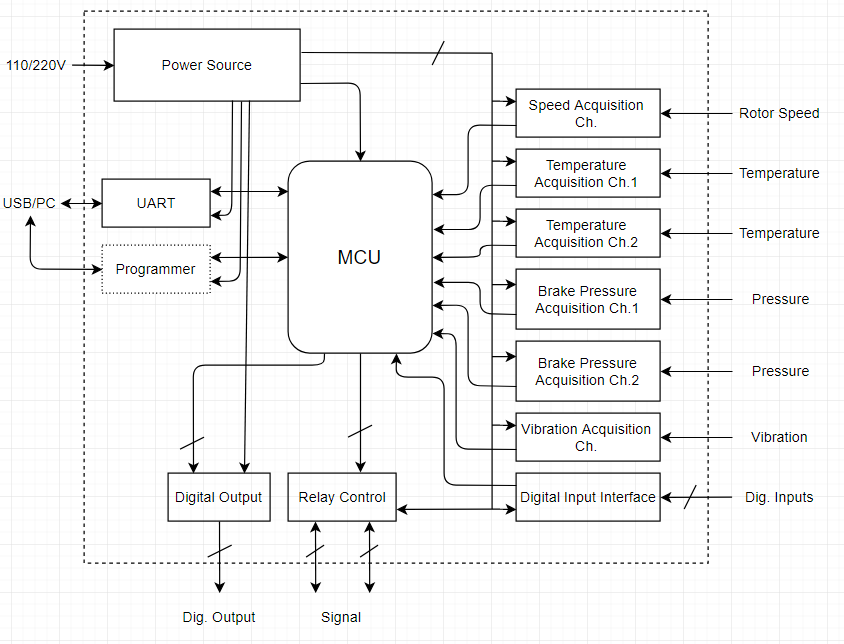
\includegraphics[scale=0.8]{figuras/fig-hardwareProject}
		\caption{Hardware Project Architecture \cite{hw-proj}}
		\label{fig:hardwareProject}
	\end{figure}
	
	\section{MCU}\label{sec:mcu-hw}

		\subsection{The choosen MCU}\label{ssec:the-choosen-mcu}

		The choosen microcontroller for the system is the \textit{ATMEGA328PB} manufactured by \textit{Microchip}.It has 32 Kb of flash memory, 1 Kb of \textit{EEPROM} (Electrically Erasable Programmable Read-Only Memory), 2Kb of \textit{SRAM} (Static Random Access Memory), 27 GPIOs, 32 general purpose registers, five flexible timer/counters, two USARTs, 8-channel 10bit ADC \cite{atmega328p-datasheet}. 
		\par
		This microncontroller is widely used in academic environment (specially after the Arduino project started, when microncontroller programming became much more feasible and reachable), and is famous for being easy and reliable to use. The \textit{ATmega328p} has eight ADC inputs with a resolution of 10 bits and more 27 GPIO ports. This microcontroller also has a UART. It is really versatile and more important it meets this project requirements, listed in Section \ref{sec:functionalRequirements}. This microcontroller will be used with a five volts supply, giving digital inputs and outputs a standard high logic level of five volts and low logic level of zero volts. The Figure \ref{fig:atmega328pb} shows the pinout of this device.

		\begin{figure}[htbp]
			\centering
			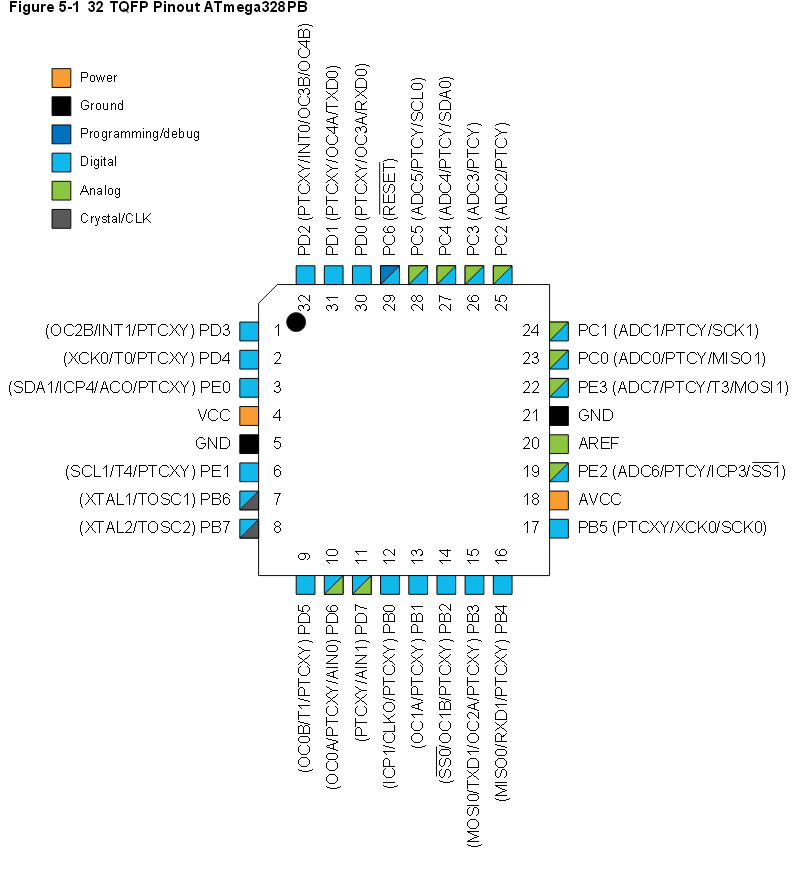
\includegraphics[scale=0.5]{figuras/fig-atmega328pb.png}
			\caption{\textit{ATmega238PB} pinout \cite{atmega328p-datasheet}}
			\label{fig:atmega328pb}
		\end{figure}
		

		\subsection{MCU circuit}\label{ssec:mcu-circuit}

		Figure \ref{fig:mcu-circuit} shows the complete complementary circuit for the MCU.

		\begin{figure}[htbp]
			\centering
			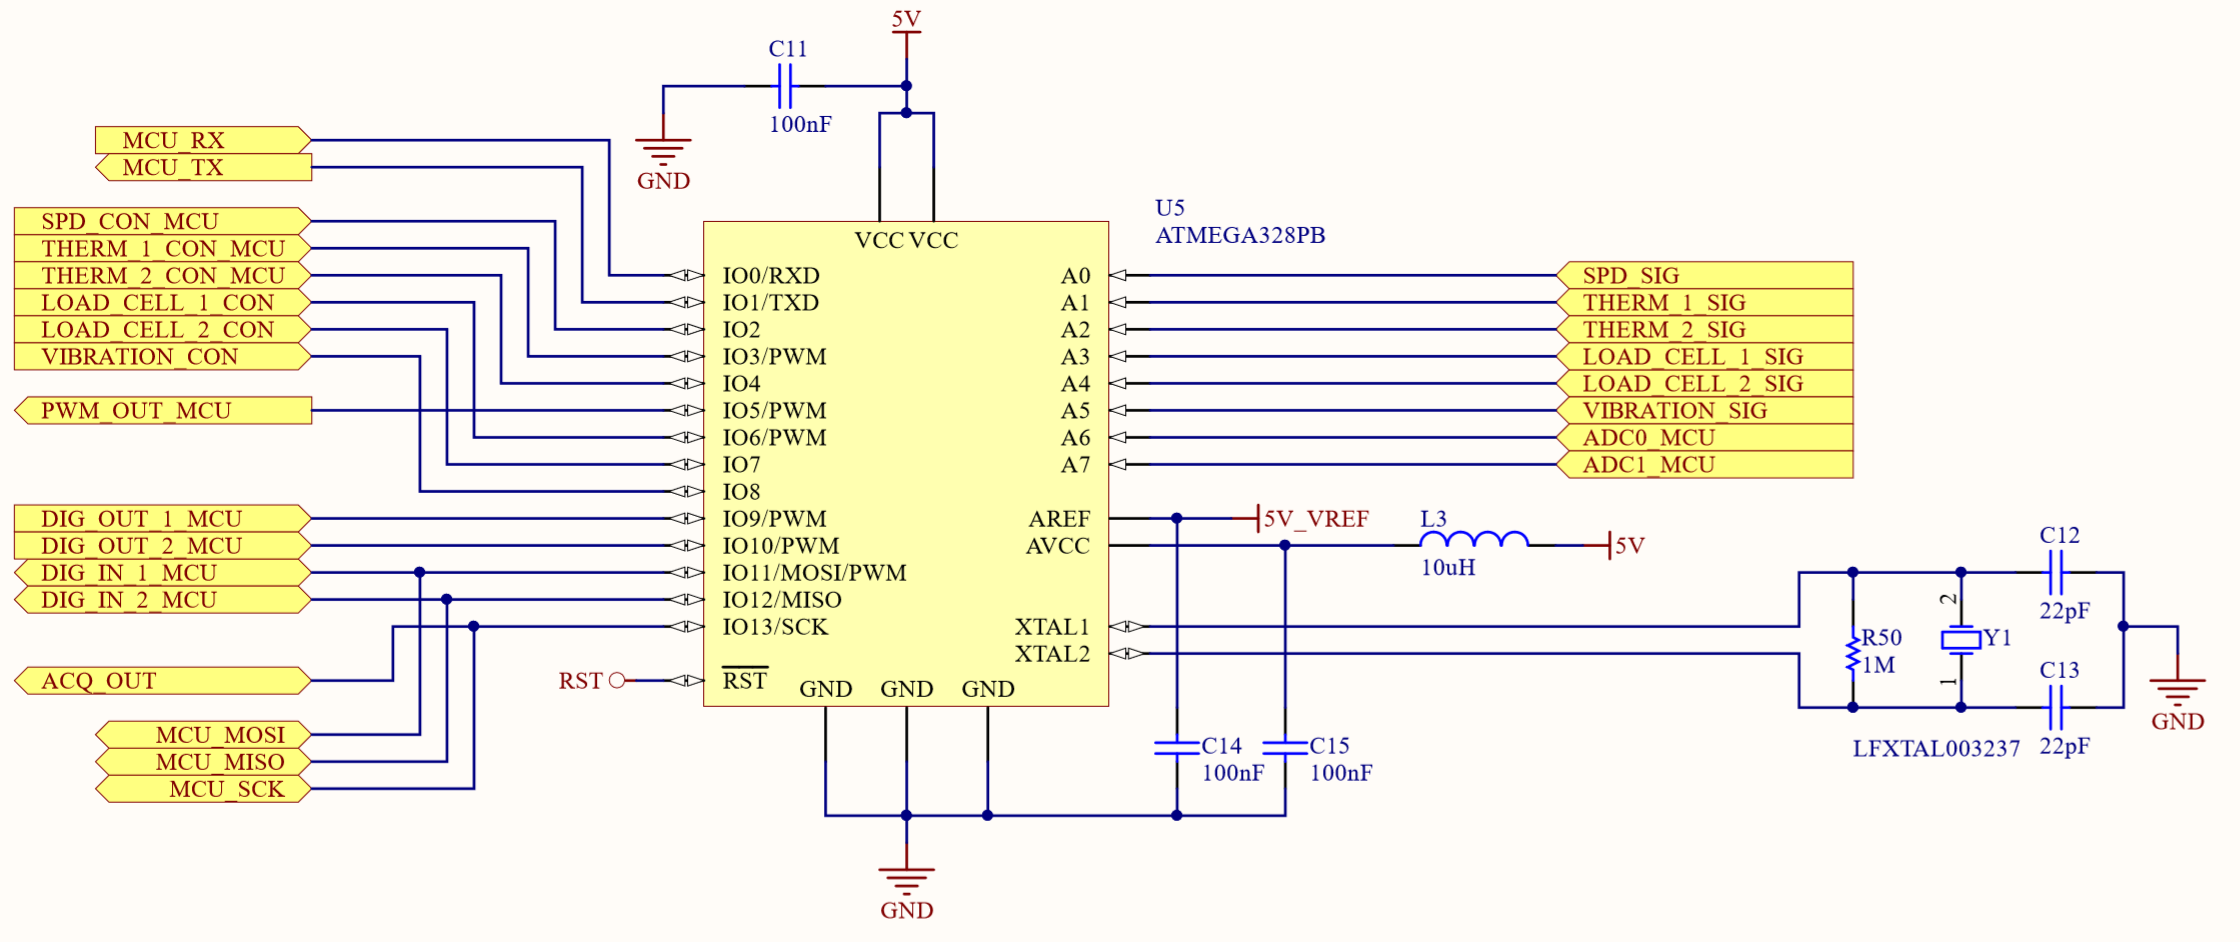
\includegraphics[scale=0.7]{figuras/fig-mcu-circuit.png}
			\caption{MCU Complete Complementary Circuit \cite{mcu-circuit}}
			\label{fig:mcu-circuit}
		\end{figure}

			\subsubsection{MCU Communication Ports}\label{sssec:mcu-com-ports}
				The ports in yellow and the RST ports are the MCU communication connections with other circuit modules, they are described as it follows.

				\begin{itemize}
					\item \textit{MCU$\_$RX (input):} This port is used for receiving the serial data from the USB/UART circuit, as it was explained in Section \ref{ssec:usb-uart-complete-circuit}.\label{itm:mcu-port-mcu-rx}
					\item \textit{MCU$\_$TX (output):} This port is used for transmitting the serial data to the USB/UART circuit, as it was explained in Section \ref{ssec:usb-uart-complete-circuit}.\label{itm:mcu-port-mcu-tx}
					\item \textit{SPD$\_$CON$\_$MCU (input):} A signal coming from the speed acquisition channel (Section \ref{ssec:ckp-sensor-detection-circuit}) that indicates whether the sensor in connected or not.\label{itm:mcu-port-spd-con-mcu}
					\item \textit{THERM$\_$1$\_$CON$\_$MCU (input):} A signal coming from the first temperature acquisition channel (Section \ref{ssec:thermocouple-sensor-detection}) that indicates whether the sensor in connected or not.\label{itm:mcu-port-therm1-con-mcu}
					\item \textit{THERM$\_$1$\_$CON$\_$MCU (input):} A signal coming from the second temperature acquisition channel (Section \ref{ssec:thermocouple-sensor-detection}) that indicates whether the sensor in connected or not.\label{itm:mcu-port-therm2-con-mcu}
					\item \textit{LOAD$\_$CELL$\_$1$\_$MCU (input):} A signal coming from the first brake pressure acquisition channel (Section \ref{ssec:load-cell-sensor-detection}) that indicates whether the sensor in connected or not.\label{itm:mcu-port-load-cell-1-mcu}
					\item \textit{LOAD$\_$CELL$\_$2$\_$MCU (input):} A signal coming from the second brake pressure acquisition channel (Section \ref{ssec:load-cell-sensor-detection}) that indicates whether the sensor in connected or not.\label{itm:mcu-port-load-cell-2-mcu}
					\item \textit{VIBRATION$\_$CON (input):} A signal coming from the vibration acquisition channel (Section \ref{ssec:accelerometer-sensor-detection-circuit}) that indicates whether the sensor in connected or not.\label{itm:mcu-port-vibration-con}
					\item \textit{PWM$\_$OUT$\_$MCU (output):} This is a PWM signal that goes from the MCU to the DAC circuit in other to control the electric engine speed (Section \ref{ssec:pwm-to-speed-reference-circuit}).\label{itm:mcu-port-pwm-out-mcu}
					\item \textit{DIG$\_$OUT$\_$1$\_$MCU (output):} First digital external output used in the circuit (Section \ref{ssec:digital-outputs}).\label{itm:mcu-port-dig-out-1-mcu}
					\item \textit{DIG$\_$OUT$\_$2$\_$MCU (output):} Second digital external output used in the circuit (Section \ref{ssec:digital-outputs}).\label{itm:mcu-port-dig-out-2-mcu}
					\item \textit{DIG$\_$IN$\_$1$\_$MCU (input):} First digital external input used in the circuit (Section \ref{ssec:digital-inputs}).\label{itm:mcu-port-dig-in-1-mcu}
					\item \textit{DIG$\_$IN$\_$2$\_$MCU (input):} Second digital external input used in the circuit (Section \ref{ssec:digital-inputs}).\label{itm:mcu-port-dig-in-2-mcu} 
					\item \textit{ACQ$\_$OUT (output):} Used to control a LED that blinks when signal acquisition is taking place.\label{itm:mcu-port-acq-out}   
					\item \textit{MCU$\_$MOSI:} Used for ISP programming (Section \ref{sssec:microcontroller-isp-programming}).\label{itm:mcu-port-mcu-mosi}
					\item \textit{MCU$\_$MISO:} Used for ISP programming (Section \ref{sssec:microcontroller-isp-programming}).\label{itm:mcu-port-mcu-miso}
					\item \textit{MCU$\_$SCK:} Used for ISP programming (Section \ref{sssec:microcontroller-isp-programming}).\label{itm:mcu-port-mcu-sck}
					\item \textit{SPD$\_$SIG: (input):} Analog input for the speed signal (Section \ref{ssec:ckp-signal-conditioning-circuit}).\label{itm:mcu-port-spd-sig}
					\item \textit{THERM$\_$1$\_$SIG: (input):} Analog input for the first temperature signal (Section \ref{ssec:thermocouple-signal-conditioning}).\label{itm:mcu-port-therm-1-sig}
					\item \textit{THERM$\_$2$\_$SIG (input):} Analog input for the second temperature signal (Section \ref{ssec:thermocouple-signal-conditioning}).\label{itm:mcu-port-therm-2-sig}
					\item \textit{LOAD$\_$CELL$\_$1$\_$SIG (input):} Analog input for the first brake pressure signal (Section \ref{ssec:load-cell-signal-conditioning}).\label{itm:mcu-port-load-cell-1-sig}  
					\item \textit{LOAD$\_$CELL$\_$2$\_$SIG (input):} Analog input for the second brake pressure signal (Section \ref{ssec:load-cell-signal-conditioning}).\label{itm:mcu-port-load-cell-2-sig} 
					\item \textit{VIBRATION$\_$SIG (input):} Analog input for the vibration intensity signal (Section \ref{ssec:accelerometer-signal-conditioning-circuit}).\label{itm:mcu-port-vibration-sig}
					\item \textit{ADC0$\_$MCU (input):} This port is not used and an internal MCU pull-up resistor is used.\label{itm:mcu-port-adc0-mcu}
					\item \textit{ADC1$\_$MCU (input):} This port is not used and an internal MCU pull-up resistor is used.\label{itm:mcu-port-adc1-mcu}
					\item \textit{RST (input):} This is the reset connection for the MCU, used to reset the MCU using ISP programming.\label{itm:mcu-port-rst}
				\end{itemize}
		
			\subsubsection{MCU Power Ports}\label{sssec:mcu-power-ports}
				The MCU power ports are described as it follows, each power port funcion was taken from the components datasheet \cite{atmega328p-datasheet}. All voltage supplies have a 100nF decoupling capacitor also recommended by the MCU datasheet.

				\begin{itemize}
					\item \textit{VCC: } This is the main voltage supply port for the MCU, as mentioned in Section \ref {ssec:the-choosen-mcu} the MCU will be powered up with a 5V supply. More details of this supply line in Section \ref{sssec:5v-supply}.\label{itm:mcu-vcc}
					\item \textit{GND: } This is the ground reference for the MCU.\label{itm:mcu-gnd}
					\item \textit{AREF: } This is the analogic voltage reference for the ADC, a ADC is as good as it's voltage reference \cite{adc-good}. The net \textit{5V$\_$VREF} is internally connect to the MCU precision reference.
					\item \textit{AVCC: } This is the ADC power supply, the inductor was used to filter unwanted noise, and the usage of this inductor was based on the Arduino Uno Rev3 Schematic \cite{arduino-rev3-schematic}.\label{mcu-avcc}
				\end{itemize}

			\subsubsection{Crystal Oscilator Circuit}\label{sssec:mcu-crystal-oscilator}

				The MCU datasheet indicates the use of a external oscilation crystal, the additional components to the crystal were based on the Arduino Uno Rev3 \cite{arduino-rev3-schematic}.
	\section{Temperature Acquisition Channel}

	\subsection{Thermocouple Type and Signal}	
			
	 For this project it was defined that thermocouples of type K (formed by the junction of two metal leagues: Alumel and Cromel) would be used in this project. This is because this specific type of thermocouple has a wide range of operation (-200$^{\circ}$C - 1200 $^{\circ}$C), so according to the requirements they are never too close from the boundary values, a thermocouple of type T or even a type J would not be suitable. Other appealing factor is that this type of thermocouple is quite common so getting eventual replacements would be easier, in comparisson with type E thermocouples.

	\subsection{Thermocouple Signal Conditioning}
	
	As mentioned in sub-section \ref{ssec:thermocouple}, besides amplification and linearization, the thermocouple signal also needs it's cold junction temperature difference compensation. There is an integrated solution from \textit{Analog Device} called AD8495, this IC functional diagram is displayed on Figure \ref{fig:ad8495-functional-block}.
	
		\begin{figure}[htbp]
			\centering
				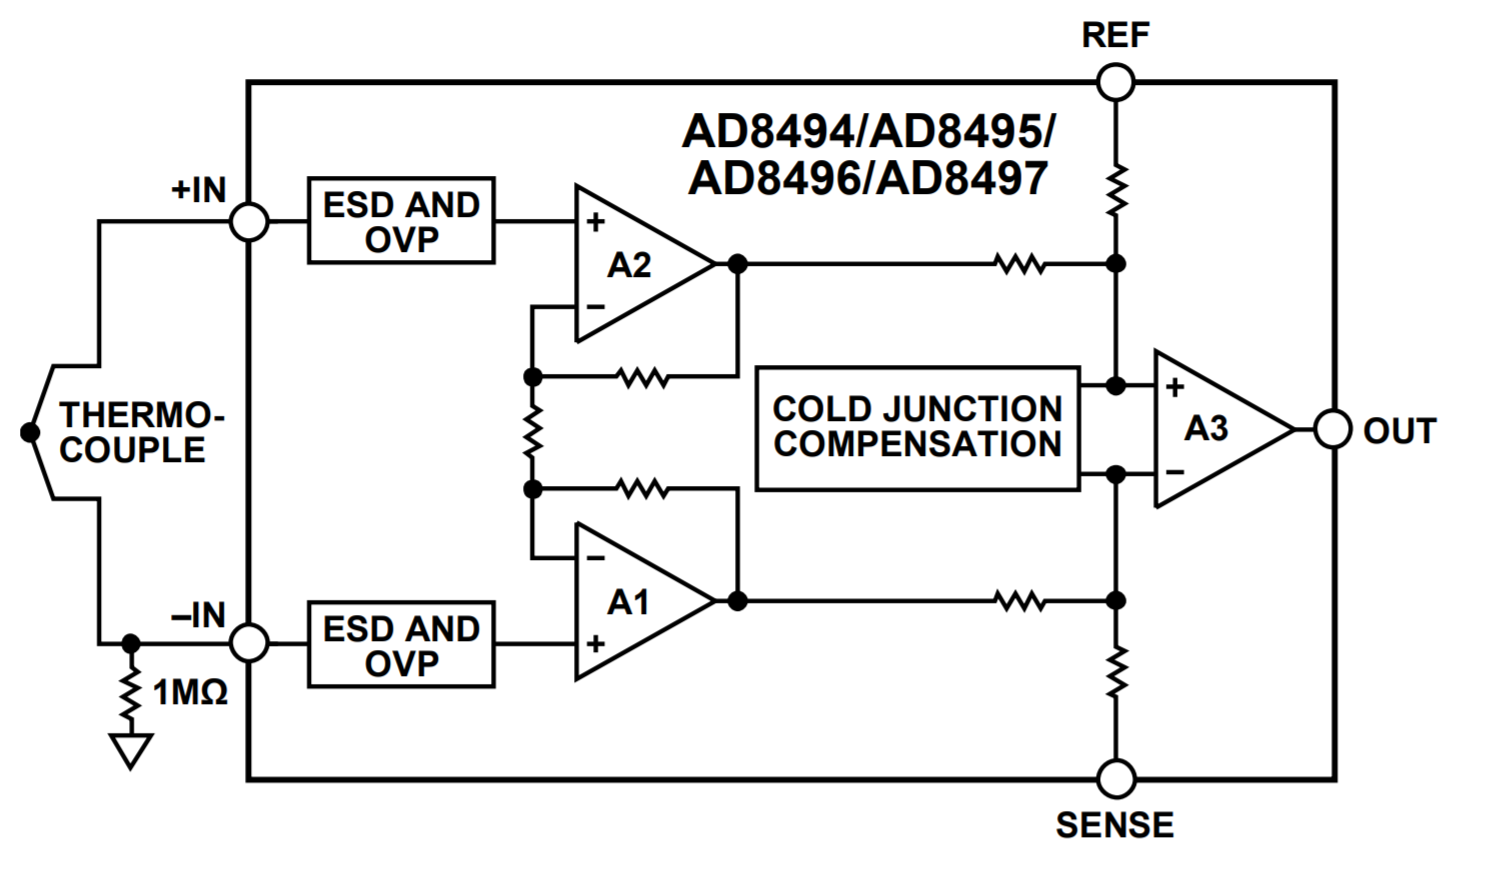
\includegraphics[scale=0.65]{figuras/fig-ad8495-functional-block}
			\caption{AD8495 Functional Block Diagram \cite{ad8495-functional-block}}
			\label{fig:ad8495-functional-block}
		\end{figure}
		
	This IC produces a linearized output with a fixed gain of $5mv\/^\circ}$C, it is a quite practical solution as it can be powered with single-supply voltage source and it's output saturates to the power supply voltage if the thermocouple is disconnected \cite{ad8495-datasheet}.
	
	\subsection{Input Protection and Filtering}\label{ssec:ad8495InputProtectionAndFiltering}
	
	Although this IC already has overvoltage and ESD protection, thermocouples tips can pick a load of unwanted noise and transients. Hence, additional protection and external filtering is also recommended by \cite{two-ways-thermocouple}. First thing to do is to add current-limint series resistors, the drawback is doing that is that resistors in the circuit net increases the overall noise. This type of noise is called Johnson-Nyquist Thermal Noise or more commonly just by Johnson Noise, thermal agitation of electrons in a resistor gives rise to random fluctuations in the voltage across its terminals \cite{romero1998johnson}. Moreover, it can be calculated using the following Equation \ref{eqn:johnson-noise} where K is the Boltzamann's constant $1.38 \cdot 10^{-23}$, R is the resistance in ohms $(\Omega)$ and T the temperature in kelvin (~300K at room temperature) \cite{sensors2000}.
	
		\begin{equation}\label{eqn:johnson-noise}
			Noise (nv\/\sqrt{Hz}) = \sqrt{4 \cdot K \cdot R \cdot T \cdot 10^{9}}
		\end{equation}
		
	Because the protection circuit includes two equal resistors, whose noise is uncorrelated, that is, the two noise sources are independent of each other—the above result must be multiplied by the square root of 2 (the root sum square of the two noise voltages) and it is considered as a general rule design to tolerate additional Johnson Noise from 10 to 30$\%$ to the amplifier IC \cite{sensors2000}. \cite{two-ways-thermocouple} suggests using current-limiting resistors of 10$k\Omega$, according to the AD8495 datasheet \cite{ad8495-datasheet}, the choosen amplifier (AD8495) has a voltage noise density of 32nV$\/ \sqrt{Hz}$. Combining this resistors noise with the amplifier noise will produce a overall noise of 36.85nV$\/\sqrt{Hz}$, which is just 13$\%$ above the amplifier's own noise. Additional protection can be achieved using external protection diodes as on Figure \ref{fig:externalProtectionDiodes}.
	
		\begin{figure}[htbp]
			\centering
				\includegraphics[scale=0.65]{figuras/fig-externalProtectionDiodes}
			\caption{External Protection Diodes \cite{externalProtectionDiodes}}
			\label{fig:externalProtectionDiodes}
		\end{figure}
		
	A Transient Voltage Suppression Diode (TVS) can be used to protect the inputs from differential input overvoltage, considering a bidirectional TVS with a 5V breakdown voltage, the device will theoretically limit the differential voltage between 5V and -5V, the AD8495 has overvoltage protection from -25V to 20V when powered with 5V, so this will successfully protect the amplifier inputs. It is also interesting to clamp each input to the supply rails using, this is best done using Schottky diodes, this type of diode operates the same way as standard diodes but have faster response and lower forward voltage. Schottky diodes have a foward voltage of approximately 200mV, if the supply rails are of 5V and 0V, a pair of diodes connected in the same way of Figure \ref{fig:externalProtectionDiodes}, the inputs will be clamped on -200mV and 5200mV, protecting the input.
	\par
	With the overloads protection done, another important feature to do is to filter unwanted signals in the inputs to avoid them to be amplified later, this is done by filtering Radio Frequency Interference (RFI), signal lines (specially for low level signals) are quite susceptible to RF interference \cite{analogDevDesignersGuide}. Interference that occurs on both lines are usually reduced by the amplifiers own common-mode rejection filter, but only on a limited bandwidth, also the in-amp rectifier cannot filter differential RF interference. The choosen amplifier (AD8495) has a -3dB bandwidth at 25kHz, \cite{two-ways-thermocouple} suggests setting a common-mode cutoff filter frequency at 16kHz (in order to guarantee the input signal within the 25kHz bandwidth). The standard circuit for the RFI filter is displayed on Figure \ref{fig:rfi-standard-filter}, resistors R1 and capacitors C1 are used to filter common-mode interference and it is important that state that $R1_{a}$=$R1_{b}$ and $C1_{a}$=$C1_{b}$. Capacitor C2 is connected across the bridge output to reduce any common-mode rejection errors due to the components mismatch, that way filtering any differential interference. C2 is usually choosen to be ten times larger than C1 \cite{ad8495-datasheet}.
	
		\begin{figure}[htbp]
			\centering
				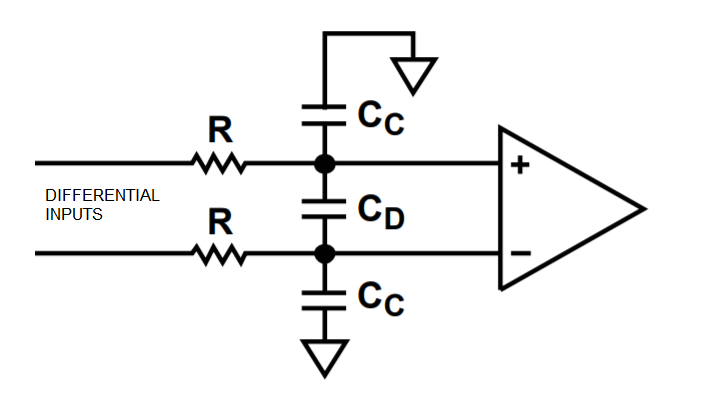
\includegraphics[scale=0.65]{figuras/fig-rfi-standard-filter}
			\caption{RFI filter circuit \cite{fig-rfi-standard-filter}}
			\label{fig:rfi-standard-filter}
		\end{figure}

	The -3dB common-mode bandwidth of this filter from Figure \ref{fig:rfi-standard-filter} is given by Equation \ref{eqn:bw-common-mode-rejection-filter} \cite{analogDevDesignersGuide}.

		\begin{equation}\label{eqn:bw-common-mode-rejection-filter}
			BW_{CM}=\frac{1}{2 \cdot \pi \cdot R1 \cdot C1}
		\end{equation}
	
	The -3dB differential bandwidth of this filter from Figure \ref{fig:rfi-standard-filter} is given by Equation \ref{eqn:bw-differential-rejection-filter} \cite{analogDevDesignersGuide}.
	
		\begin{equation}\label{eqn:bw-differential-rejection-filter}
			BW_{DIFF}=\frac{1}{2 \cdot \pi \cdot R1 \cdot \left( 2 \cdot C2 + C1 \right)}
		\end{equation}
		
	Using the values for the current limiting resistors (10k$\Omega$), Equation \ref{eqn:bw-common-mode-rejection-filter} and the suggested cutoff frequency of 16kHz \cite{two-ways-thermocouple}, it is possible to calculate a value of 1nF for C1. Choosing a C2 value ten times larger than C1 implies on using a C2 value of 10nF, that used on Equation \ref{eqn:bw-differential-rejection-filter} will produce a differential interference filter cutoff frequency of 1.3kHz.
		
	\subsection{Thermocouple Sensor Detection}
		
	A important feature of any acquisition system is to detect when a sensor is disconnected from the the acquisition system input \cite{o2011pressure}, because a signal acquisition circuit without the signal source will generate outputs that are uncorrelated to what the system was designed to measure/sense on the outside world. The AD8495 has a quite useful feature \cite{ad8495-datasheet}, it offers open thermocouple detection, the inputs of the AD8495 are PNP type transistors, which means that the bias current always flows out of the inputs. This way, the input bias current drives any unconnected output high, which saturates the output to the maximum possible reading, being in this case 1000$^{o}$C or 5V (considering the fixed 5mv$\/ ^{o}$C gain. In Section \ref{sec:functionalRequirements}, it was defined that the system must measure temperatures up to 600$^{o}$C, with the fixed gain of 5mv$\/^{o}$ this means an output voltage of 3V. So the so called \textit{Thermocouple Sensor Detection} must be able to detect whenever the output exceeds 3V. In order to do that, the circuit displayed in Figure \ref{fig:thermocouple-sensor-detection} was designed.
	
		\begin{figure}[htbp]
			\centering
				\includegraphics[scale=0.65]{figuras/fig-thermocouple-sensor-detection}
			\caption{Thermocouple Sensor Detection Circuit}
			\label{fig:thermocouple-sensor-detection}
		\end{figure}
		
	The diode D1 is a 3V9 zener diode, added this with the transistor Q1 (BC548) which has a typical \textit{Base-Emitter On Voltage} of 660mV \cite{bc548 }, whenever the input voltage (AD8495 output voltage) exceeds 4.56V, it will turn Q1 on. When Q1 is on the output will be the 5V from the source, when Q1 is off (voltage not exceeding the 4.56V threshold) the \textit{pull-down} resistor at Q1 emitter will take the output voltage to 0V meaning there is no disconnection issue. The other 10k$\Omega$ resistor is a \textit{pull-down} used to guarantee that the base-emitter voltage is 0V if there is no voltage on the AD8495 output. The 4.7k$\Omega$ resistor is a current limiting resistor used just to make sure just a small amount of current will be driven from the AD8495 output.

	\substion{Final Circuit}
	

	\section{Brake Pressure Acquisition Channel}\label{sec:brake-pressure-acquisition-channel}

\subsection{Load Cell Signal}\label{ssec:load-cell-signal}

	A very influential parameter in a braking system is the pressure that the brake exerts on the rotor. Pressure is a magnitude measured in Pascal and can be expressed by the force ratio by the area. There are some sensors based on the piezoelectric effect, but the most accurate way to measure force is by using load cells.
	\par
	Load cells have very low output levels, of the level of 2mV/V, and therefore an amplification is fundamental. It is not necessary to know the nature of the strain gauges when a load cell is being calibrated since generally the manufacturers provide a calibration curve based on the signals $V_{O}$ and $V_{EX}$ of the Figure \ref{fig:wheatstone}, it is worth noting that these signals can not have the same reference, otherwise it will not be possible to excite the wheatstone bridge correctly.
	\par
	The most common way to amplify the signal of a load cell is using a instrumentation amplifier. Although it is a widely used configuration, assembling this amplifier using three different operational amplifiers and seven resistors as in Figure \ref{fig:instrumentation-amplifier} may make it inaccurate due to manufacturing imperfections of the components. Another factor that greatly influences the output signal of a load cell is the excitation voltage of its wheatstone bridge, if it varies too much the output will vary greatly as well, which will hamper its calibration.

\subsection{Load Cell Signal Conditioning}\label{ssec:load-cell-signal-conditioning}
		
	In order to solve these two problems there is a solution widely used in the market which is the \textit{AD8223} from Analog Devices \cite{ad8223-datasheet}, this IC is an integrated single supply instrumentation amplifier that delivers rail-to-rail output swing. Other good feature of this amplifier is that as it has a great CMRR \textit{Common-Mode Rejection Ratio} of 80dB, making it very much suitable for condionting differential pair signals (such as the one from the Load Cell as Subsection \ref{ssec:load-cell} mentions), more information of CMRR in Subsection \ref{sssec:important-features-to-consider-in-a-amplifier}. The only external component needed is a resistor $R_{G}$, as shown in Figure \ref{fig:ad8223-schematic}. This resistor will determine the gain (G) for the amplification according to the Equation \ref{eqn:ad8223-g}.
	

		\begin{figure}[htbp]
			\centering
				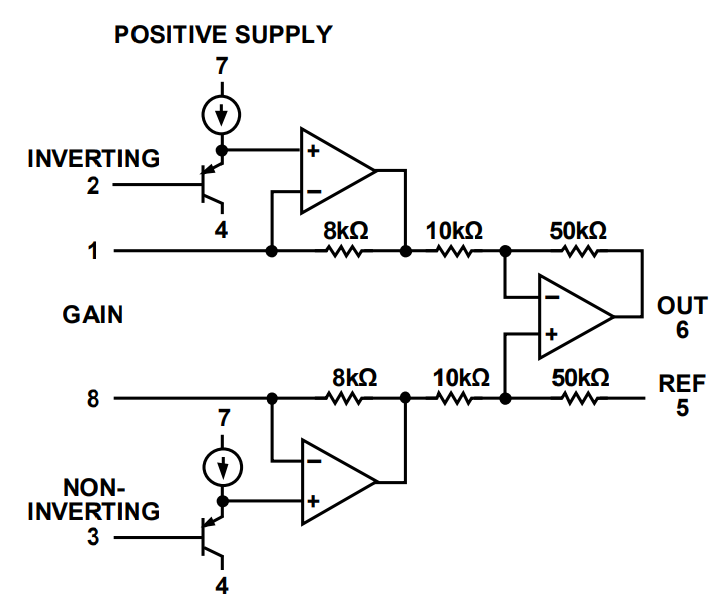
\includegraphics[scale=0.65]{figuras/fig-ad8223-functional-block.png}
			\caption{AD8223 Schematic \cite{ad8223-datasheet}}
			\label{fig:ad8223-schematic}
		\end{figure}

		\begin{equation}\label{eqn:ad8223-g}
			R_{G}=\frac{80k\Omega}{G - 5}
		\end{equation}

		Taking into account the sensitivity of 2mV/V, this means that if the cell is excited with 10V, its output will vary from 0 to 20mV. The precision of the excitation voltage will naturally affect the performance of the sensor, Section \ref{sssec:10v-reference} will explain how a precise 10V voltage reference will be achieved.
		\par
		Since the analog input of the chosen microcontroller \textit{(Atmega328)} is 0 to 5V, we may to amplify the cell output signal by a factor of 250 in order to use the most number of bits from de MCU's ADC. Using Equation \ref{eqn:ad8223-g}, to obtain a gain of amplification ratio of the ideal $R_{G}$ would be 326$\Omega$, a resistor of this value and minimal tolerance (1$\%$) is not commercially available, the closest one is 332$\Omega$. This resistor will generate a gain of 246 and cause the IC output to range from about 0V to 4.92V, using 98.4\% of the resolution of the microcontroller input. 
		\par

		Figure \ref{fig:cic-cell} shows the schematic of the load cell conditioning circuit with the AD8223.

		\begin{figure}[htbp]
			\centering
				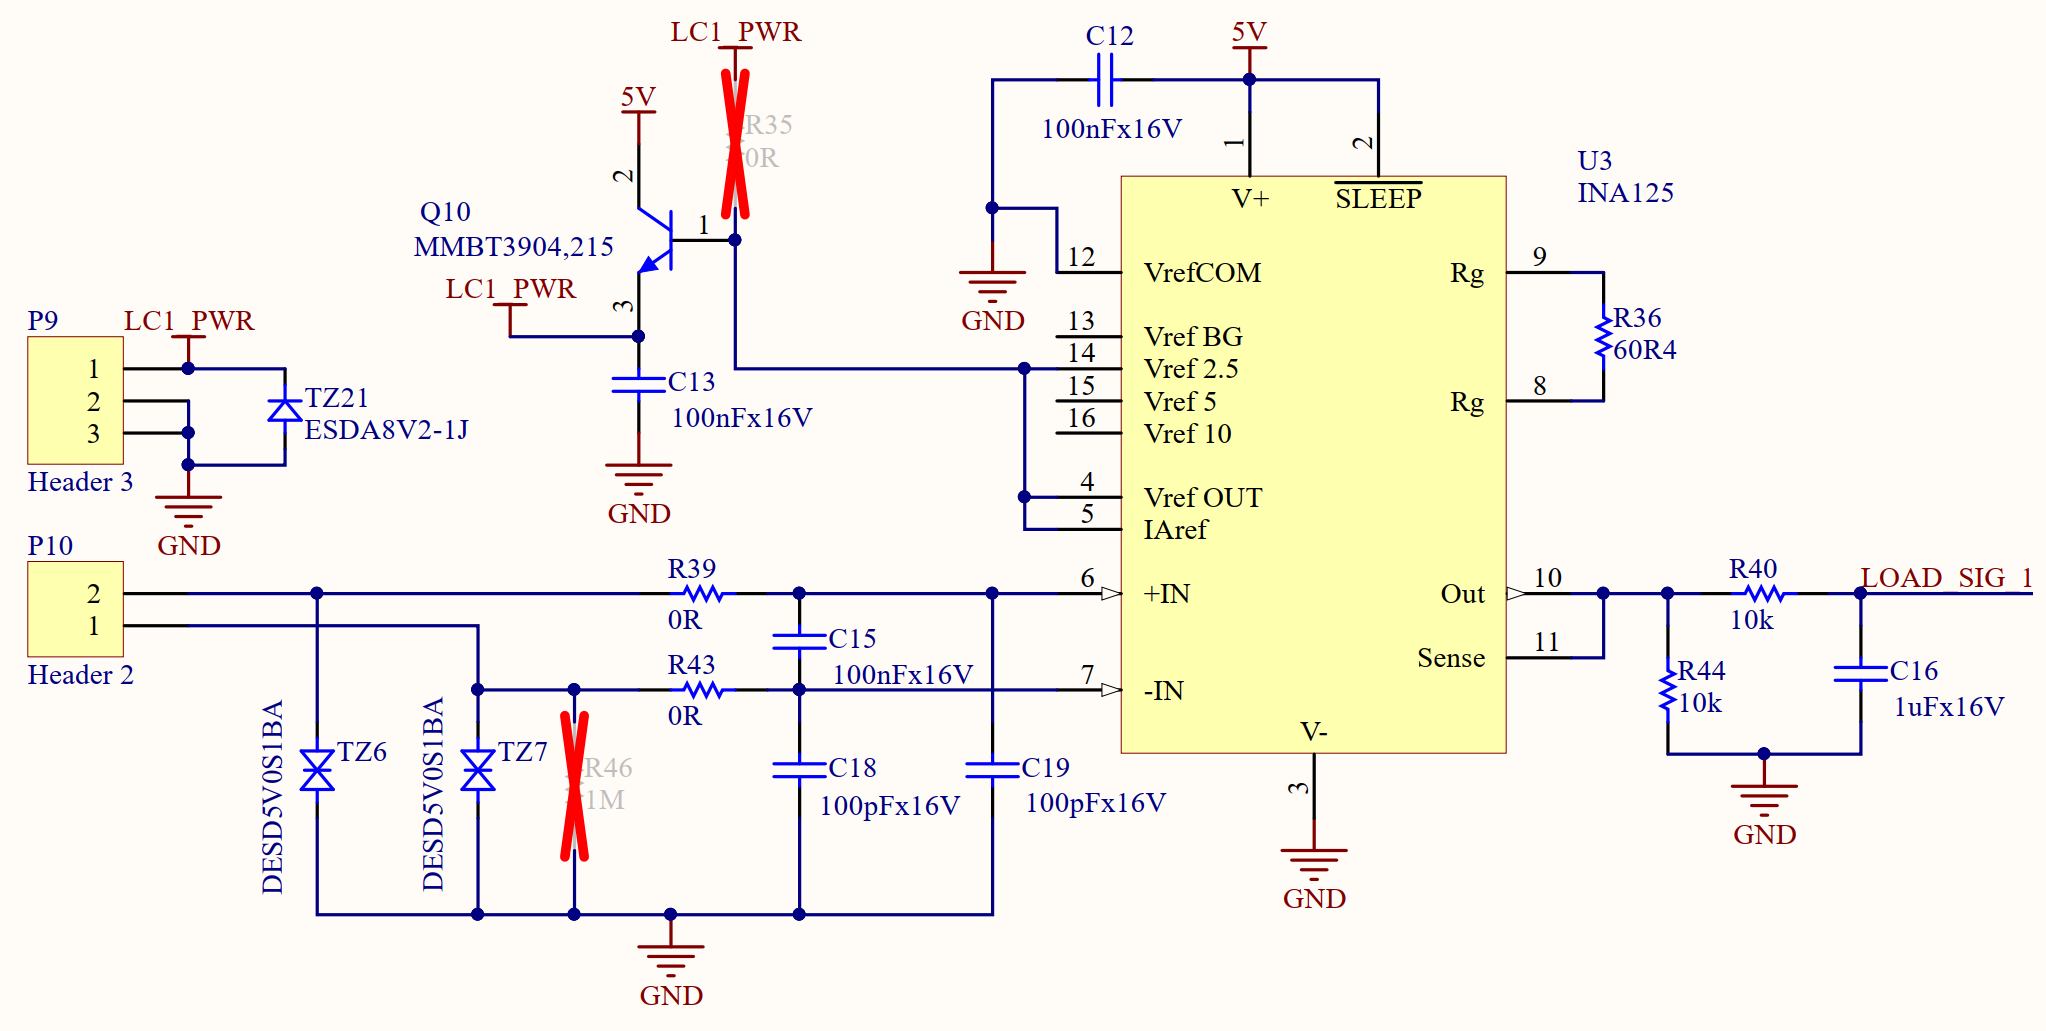
\includegraphics[scale=0.35]{figuras/fig-cic-cell.png}
			\caption{Conditioning Circuit for the Load Cell \cite{conditioning-circuit-for-the-load-cell}}
			\label{fig:cic-cell}
		\end{figure}

		It is basically the amplifier with the gain resistor plus five different types of components:
		\begin{itemize}
			\item \textbf{TVS Diode:} AD8223 datasheet says that the differential input voltage must not be greater than the supply voltage \cite{ad8223-datasheet}, hence, as the supply is 5V, a 5V TVS was added.
			\item \textbf{Decoupling Capacitor:} A decoupling capacitor is recommended by the component's datasheet \cite{ad8223-datasheet}.
			\item \textbf{Resistor R21:} Used to guarantee that if the sensor is disconnected the inverted input will be shunted to GND as according to Figure \ref{fig:ad8223-schematic} the PNP transistors in the non-inverted input will saturate the output to the supply voltage \textit{(this feature is used for detecting when the sensor is disconnected, further explained in Subsection: \ref{ssec:load-cell-sensor-detection}).}
			\item \textbf{R17 and R15:} This jumpers are used just if the need to test circuit blocks separately.
		\end{itemize}

\subsection{Load Cell Sensor Detection}\label{ssec:load-cell-sensor-detection}
	As was explained in Subsection \ref{ssec:load-cell-signal-conditioning}, with R21 the circuit will saturate the output to the supply voltage when the load cell sensor is disconnected. The circuit to detect this voltage saturation is exact the same from the one used previously on the thermocouple circuit, the circuit schematic and functional explanation can be found in Subsection \ref{ssec:thermocouple-sensor-detection}.

	\subsection{Complete Circuit}\label{ssec:load-cell-complete-circuit}
		The thermocouple complete circuit is displayed on Figure \ref{fig:load-cell-complete-circuit}.

		\begin{figure}[htbp]
			\centering
				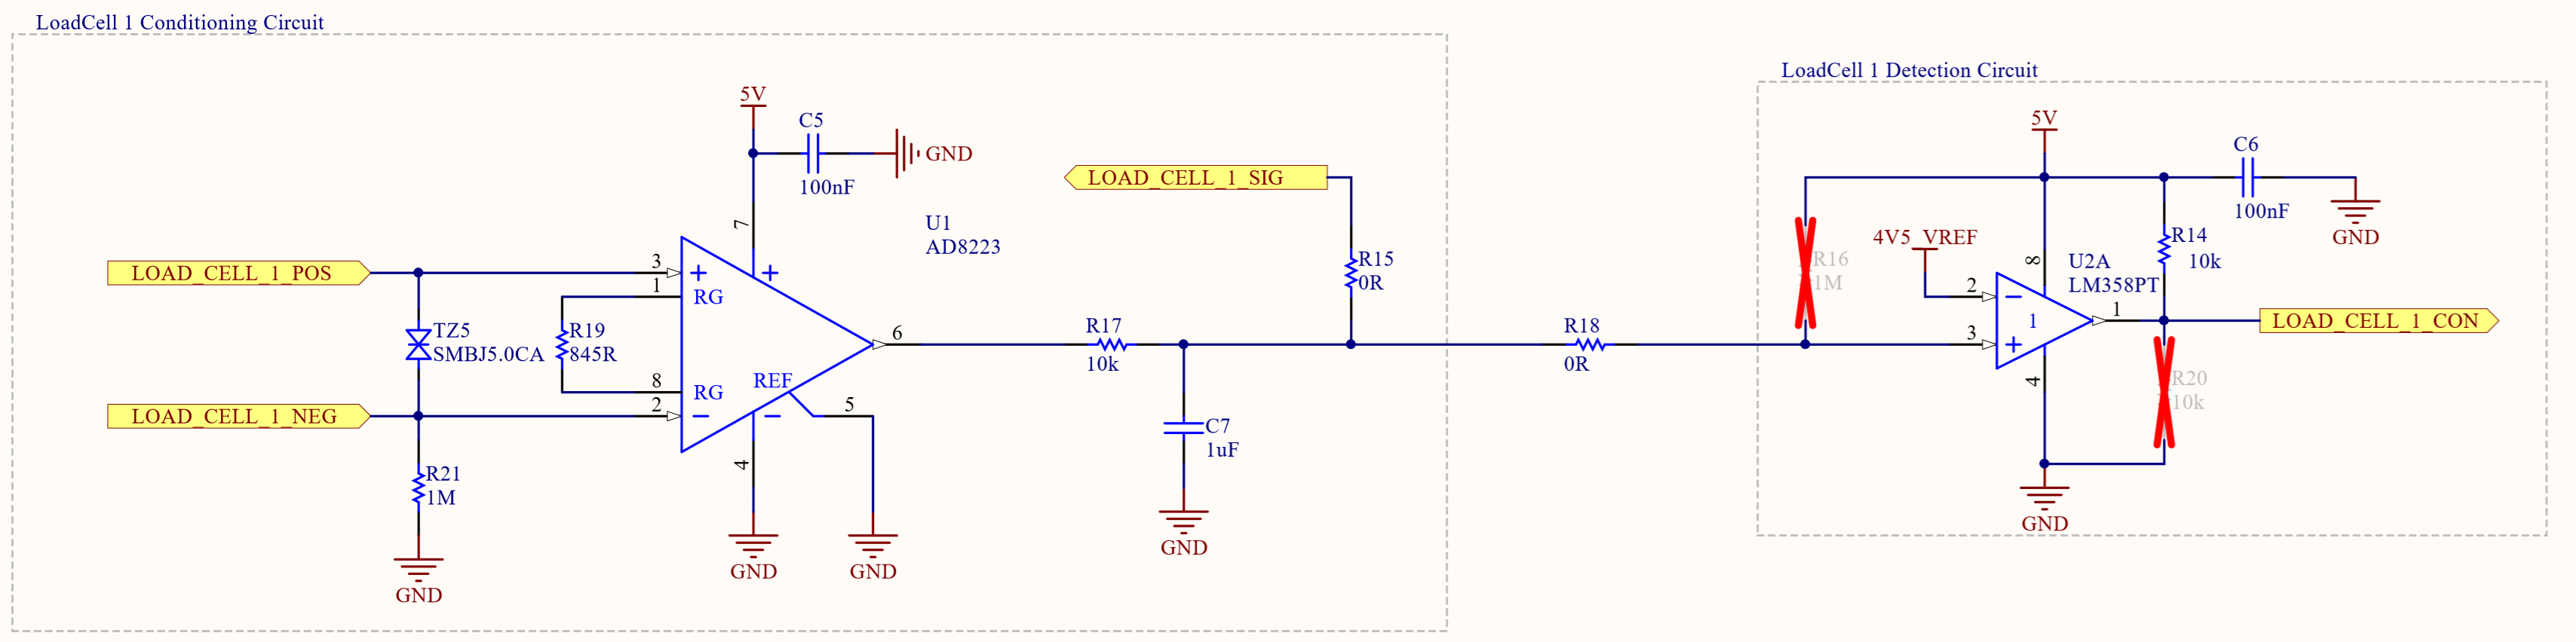
\includegraphics[scale=0.7]{figuras/fig-load-cell-complete-circuit}
			\caption{Load Cell Complete Circuit \cite{load-cell-complete-circuit}}
			\label{fig:load-cell-complete-circuit}
		\end{figure}		

		The pair composed of R17 and C7 is a LFP with a central frequency of 16Hz, used to filter any further noise including the 50/60Hz noise from AC power lines that the thermocouple wires may catch. R15 and R18 were included in case a individual circuit block test is required, both are 0R resistors (jumpers). R20 is just a pull-down to guarantee that the MCU input port will not fluctuate.	
	\section{Speed Acquisition Channel}
			

	\subsection{CKP Signal}

	\subsection{CKP Signal Conditioning}

	\subsection{CKP Sensor Detection}

	\section{Vibration Acquisition Channel}\label{sec:vibration-acquisition-channel}

\subsection{Accelerometer}\label{ssec:accelerometer-signal}
	As mentioned in Section \ref{ssec:accelerometer}, acceleration is measured in g. The choosen accelerometer for this project was the \textit{ADXL335} from \textit{Analog Devices} \cite{devices2010adxl335}. The main characteristics of this sensor are:

	\begin{itemize}
		\item It has 3 axis sensing (easy to install).
		\item Low power operation (350$\micro$A).
		\item 10,000 g shock survival.
		\item 1V8-3V3 Single-supply operation.
		\item $\pm$3g measurements.
	\end{itemize}

	When powered up with 3V3 the sensor has a linear voltage output of 0V for -3g and 3V3 for 3g. This sensor is ideal for this project, the only issue is the installation. The sensor comes in a 16-LFCSP IC (Figure \ref{fig:16lfcsp}), and this IC needs to be installed where acceleration is intended to be measured, so a additional board is necessary to install it. 

	\begin{figure}[htbp]
		\centering
			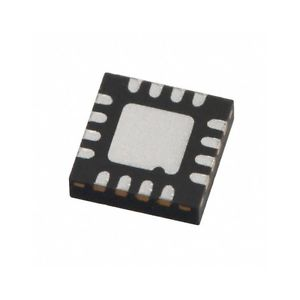
\includegraphics[scale=0.95]{figuras/fig-16lfcsp.jpg}
		\caption{16-LFCSP \cite{16lfcsp}}
		\label{fig:16lfcsp}
	\end{figure}

	The are already embdded solutions that can solve this issue, such as the \textit{Adafruit ADXL335 - 5V ready} \cite{adafruit-5v-ready}. This small (75mm x 75mm) board (Figure \ref{fig:adafruit-adxl335}) has the ADXL335 with the capacitors recommended by the datasheet, with a 3V3 voltage regulator so the board can be powererd up with 5V and with the mounting holes to fix the board in any surface, making it ideal for this project.

	\begin{figure}[htbp]
		\centering
			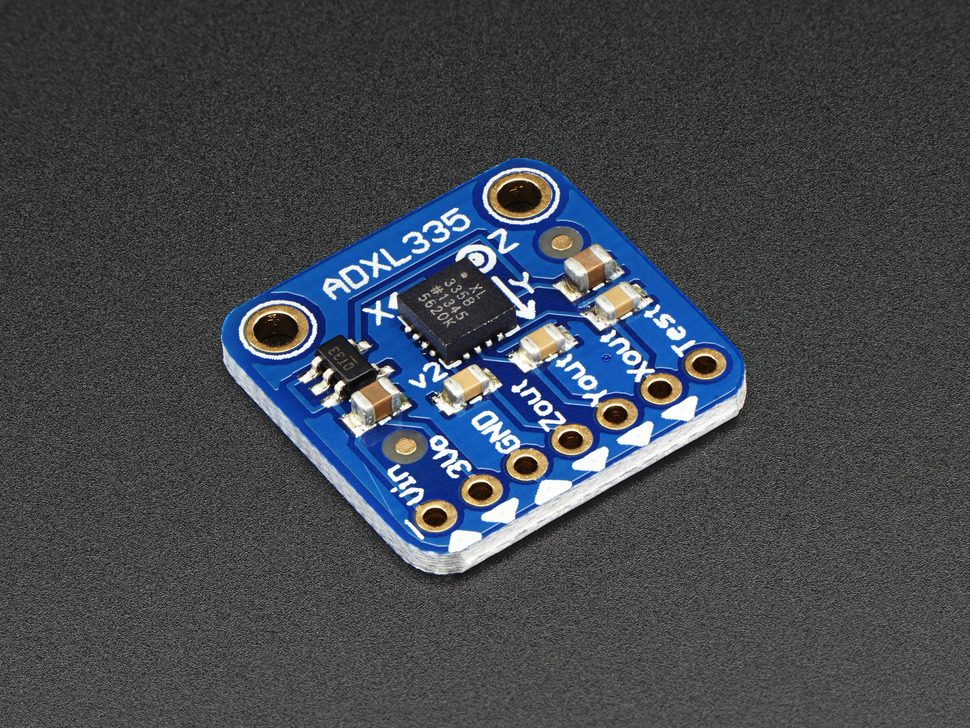
\includegraphics[scale=0.95]{figuras/fig-adafruit-adxl335.jpg}
		\caption{Adafruit ADXL335 - 5V ready \cite{adafruit-adxl335}}
		\label{fig:adafruit-adxl335}
	\end{figure}


\subsection{Signal Conditioning Circuit}\label{ssec:accelerometer-signal-conditioning-circuit}

	The ADXL335 datasheet \cite{devices2010adxl335} says that for a -3g measured acceleration the device output is of 0V and for +3g measurement it is 3V3 voltage. As said in Section \ref{ssec:the-choosen-mcu}, the choosen MCU for this project has a ADC with a 5V voltage reference, so in order to use the maximum number os bits from the ADC is it important to amplify this 0-3V3 signal to a 0-5V signal, meaning we need a circuit with a amplification gain of 1.5x.
	\par
	The sensor conditioning circuit is displayed on Figure \ref{fig:accelerometer-signal-conditioning-circuit}.

	\begin{figure}[htbp]
		\centering
			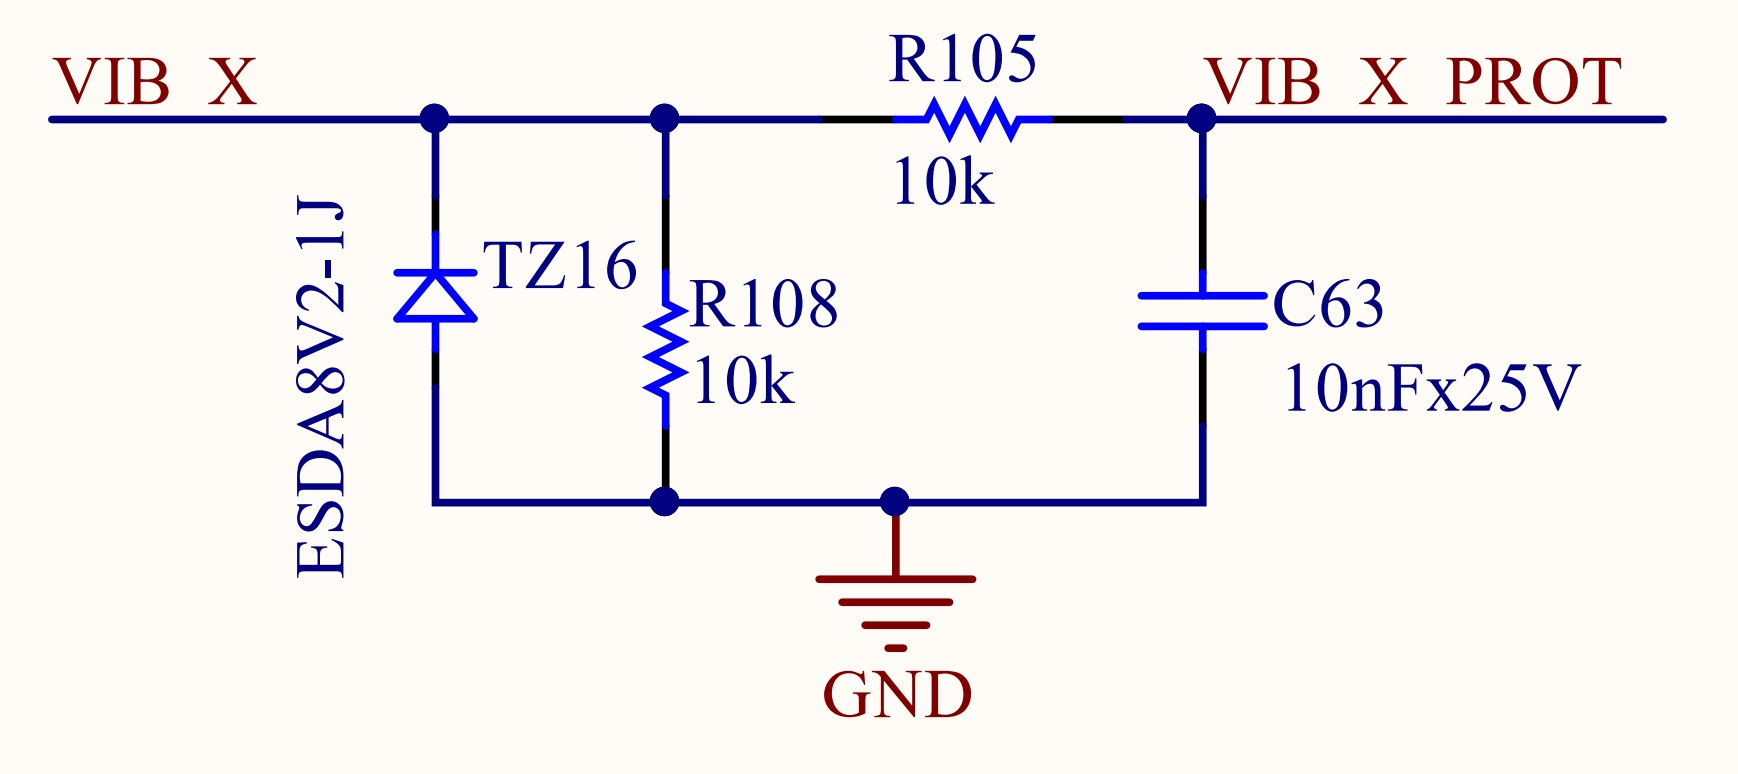
\includegraphics[scale=0.95]{figuras/fig-accelerometer-signal-conditioning-circuit.jpg}
		\caption{Accelerometer Signal Conditioning Circuit \cite{accelerometer-signal-conditioning-circuit}}
		\label{fig:accelerometer-signal-conditioning-circuit}
	\end{figure}


	The circuit is composed of three stages: protection, amplification and post-filtering. 

	\begin{itemize}
		\item \textbf{First Stage} \textit{(protection)}: Composed of a TVS diode with a standoff voltage of 3V3 (same as the sensor maximum normal output voltage level, check Item \ref{itm:tvs-standoff-voltage} from Section \ref{ssssec:tvsSelection}) and a LPF with a cutoff frequency of approximately 1.6kHz (enough to filter most ESD, check Section \ref{sssec:lowPassFilterTransientProtection}). 

		\item \textbf{Second Stage} \textit{(amplification)}: The second stage is composed by a simple non-inverting amplifier with a gain of 1.5x, to achieve this gain the resistors were choosing using Equation \ref{eqn-gain-neg-closed-loop-amp} from Section \ref{ssec:closed-loop-amplifier}. The choosen OPAMP is the \textit{MCP6001} from \textit{Microship} \cite{mcp6001-datasheet}, it was choosen for this project because it optimized to work with single-supply, has rail-to-rail input/output and has wide-bandwidth operation.

		\item \textbf{Third Stage} \textit{(post-filtering)}: The third and final stage is composed just by a LPF filter to attenuate any post amplification noise and the 50/60Hz noise interference from the power line. It has a cutoff frequency of approximately 16Hz.

	\end{itemize}

	Resistor R92 is just a jumper that was included if this circuit block is intended to be tested separately from the rest of the circuit. Resistors R96 and R94 are external pull-downs and in theory should not be mounted, they were included in the layout just in case this pull-downs become needed and then a new PCB layout would not be necessary. Capacitor C43 is just a decoupling capacitor for the amplifier supply recommended by the component datasheet \cite{mcp6001-datasheet}.

\subsection{Sensor Detection Circuit}\label{ssec:accelerometer-sensor-detection-circuit}

	As mentioned in Section \ref{ssec:accelerometer-signal}, the choosen solution for the accelerometer \textit{(Adafruit ADXL335 - 5V ready)} has a integrated 3V3 voltage regulator. In Figure \ref{fig:adafruit-adxl335} it is possible to see that the 3V3 voltage output from the voltage regulator has a connection point on the board. Hence, if a wire is connected to this point and to the main circuit board, whenever this point does not have 3V3 voltage the sensor is disconnected. Moreover, the detection circuit just need to detect when the net is in 0V or 3V3.
	\par
	The detection circuit can be seen in Figure \ref{fig:accelerometer-sensor-detection-circuit}, TZ16 is TVS diode with a standoff voltage (Item \ref{itm:tvs-standoff-voltage} from Section \ref{ssssec:tvsSelection}) of 3V3 used to protect the circuit net without interfering with it's signal. Resistor R99 is pull-down resistor, used to guarantee that the the mosfet will be not conduct current when there is no input, sensor disconnected, and the voltage on the \textit{VIBRATION_CON} net will go to 5V. R98 and C46 form a first order LPF with a cutoff frequency of aproximately 16Hz, and as a sensor disconnection process is not that fast it will filter any interference and also the noise from the 50/60Hz power lines. Finally there is R100, this is a pull-up resistor that will hold the voltage on the output to 5V when the mosfet is not polarized, sensor disconnected.

	\begin{figure}[htbp]
		\centering
			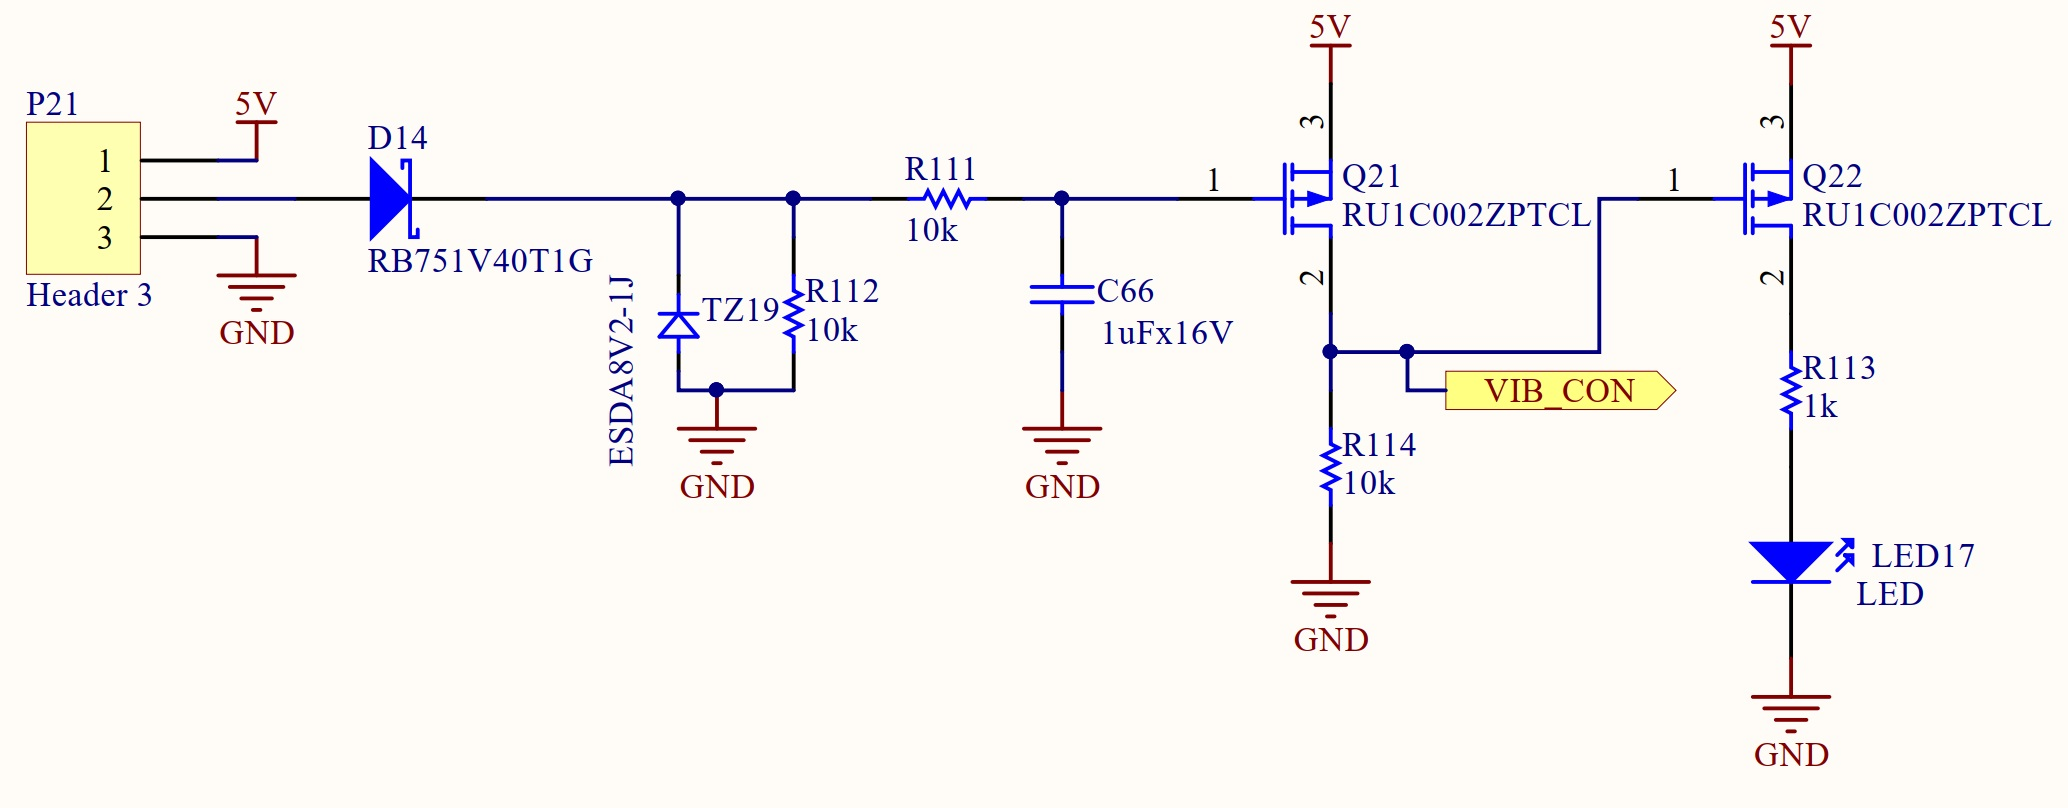
\includegraphics[scale=0.95]{figuras/fig-accelerometer-sensor-detection-circuit.jpg}
		\caption{Accelerometer Sensor Detection Circuit \cite{accelerometer-sensor-detection-circuit}}
		\label{fig:accelerometer-sensor-detection-circuit}
	\end{figure}
	\section{Speed Reference Output Channel}

	\subsection{Speed Control}
		\par
		For the braketests, somethings as important as measuring the speed of the rotor is controlling it, as mentioned in Subsection \ref{ssec:lowerLayerlHardware}. The rotor speed can be controlled in two ways:
			\begin{itemize}
				\item First way is the deceleration of the rotor with the aid of the brake system using the brake pads.
				\item Second way of controlling it by accelerating the rotor with the aid of the electric engine.
			\end{itemize}
		The electric engine used is a alternate current three-phase type, it in order to control it's speed a frequency inverter was used. The frequency inverter has many different controlling interfaces that lead to manipulating the three-phase electric system in order to control the engine's rotationary speed.
		\par
		In this project the frequency inverter used was the \textit{Weg CFW-08} \cite{wegCFW08Manual}, one way of controlling the speed of the rotor using this device is by using it's analog input, it can be configured as a notch to ten volts input that has a linear proportion to the the output frequency that goes to the engine, that way the problem to figure out in this solution is how to implement a analog output from a microcontroller that only has digital outputs.

		\begin{figure}[htbp]
			\centering
				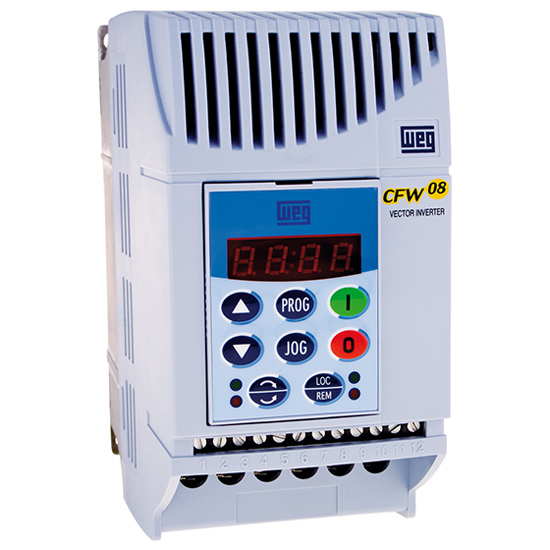
\includegraphics[scale=0.4]{figuras/fig-wegCFW08}
			\caption{Weg CFW-08 Frequency Inverter \cite{fig-wegCFW08}}
			\label{fig:wegCFW08}
		\end{figure}

	\subsection{Filter characteristics definition}\label{ssec:filterCharacteristicsDefinition}
		\par
		Fortunately the microcontroller has pre-configured PWM \textit{(Pulse Width Modulation)}, as explained in Subsection %\ref{ssec:pulseWidthModulation}
, a PWM signal can encode a analog voltage value proportional to it`s duty cycle, and this is usually done with the aid of a low pass filter that will extract this analog voltage from the PWM signal. As said in the previous paragraph the frequency inverter used in this project is the \textit{Weg CFW-08}, and it's analog input has a zero to ten voltage input with eight bits of resolution. We can calculate the minimal voltage difference that will change the output frequency of the device using Voltage, in which $\delta V$ is the minimal voltage difference, $V_{max}$ is the maximum voltage and \textit{"n"} is the number of bits of the input resolution.

			\begin{equation}\label{eqn:minVoltage}
				\delta V=\frac{V_{max}}{2^{n}}
			\end{equation}
	
		As mentioned in Section \ref{sec:mcu}, the choosen MCU has a five volts high logic level, so a five volts PWM output will need to be amplificated with a gain (k) of two in order to best the zero to ten volts input from the frequency inverter. As a consequence of that amplification the $\delta V$ from the Equation \ref{eqn:minVoltage} will be also amplificated with this gain (k) of two. This way Equation \ref{eqn:minVoltage} will me modified to consider this gain (k) as Equation \ref{eqn:minVoltage2} shows.

			\begin{equation}\label{eqn:minVoltage2}
				\delta V=\frac{V_{max}}{k \cdot 2^{n}}
			\end{equation}

		According to \cite{alter2008pwm}, converting a PWM signal to a analog voltage generates a constant voltage ripple, in our case the maximum ripple is the $\delta V$ from Equation \ref{eqn:minVoltage2}. Equation \ref{eqn:attenuation} \cite{metivier2013pwm} gives the necessary $\frac{dB}{decade}$ attenuation to guarantee a PWM converted signal desired ripple.

	 		\begin{equation}\label{eqn:attenuation}
				A_{dB}=20\cdot log \left( \frac{V_{RIPPLE}}{V_PWM} \right) 
			\end{equation}
	
		And Equation \ref{eqn:LPFcuttoffFrequency} \cite{metivier2013pwm}, is used to calculate the maximum needed cuttoff frequency for the further to be designed LPF \textit{Low-Pass-Filter} in order to convert the PWM signal to a analog voltage. This cutoff frequency can not be to much smaller than the one calculated otherwise this will have negative consequences to the output signal \cite{keim2016pwm}. The slope value is the filter slope and for first order filters and second order filters this slope value is equal respectively to 20dB/decade and 40dB/decade \cite{metivier2013pwm}.
	
			\begin{equation}\label{eqn:LPFcuttoffFrequency}
				f_{c}=f_{PWM} \cdot 10^{-\frac{A_{dB}}{Slope}}
			\end{equation}

		It is possible to combine all this equations into one single equation to calculate the needed cutoff frequency, is this done in Equation \ref{eqn:LPFcuttoffFrequency2}.

			

			\begin{equation}\label{eqn:LPFcuttoffFrequency2}
				\begin{split}
					f_{c}=f_{PWM} \cdot 10^{-\frac{A_{dB}}{Slope}}	\\
					f_{c}=f_{PWM} \cdot 10^{-\frac{20\cdot log \left( \frac{V_{RIPPLE}}{V_PWM} \right)}{Slope}}	\\
					f_{c}=f_{PWM} \cdot 10^{-\frac{20\cdot log \left( \frac{\frac{V_{max}}{k \cdot 2^{n}}}{V_PWM} \right)}{Slope}}	\\
					Knowing:	\\
					V_{max}=V_{PWM} \cdot k	\\ x \cdot log \left( A \right) =  log \left( A^{X} \right) \\
					10^{log \left( A \right) } = A	\\
					So:	\\
					f_{c}=f_{PWM} \cdot  2^{\frac{20 \cdot n}{Slope}}
				\end{split}
			\end{equation}

	
		As shown in Appendix \ref{app:microCode}, the PWM frequency was defined so $f_{PWM}=62.5kHz$, also $n=8$ and as according to \cite{metivier2013pwm}, a second order LPF is better for converting a PWM signal to voltage and it has by default $Slope=-40dB/decade$, using Equation \ref{eqn:LPFcuttoffFrequency2} it is possible to calculate a maximum cutoff frequency of 3906.25Hz. 

	\subsection{Sallen-Key Low Pass Active Filter}
	
		The Sallen-Key LPF setup is probably one of the best second order filters architectures available \cite{dorfSvodoba2014}, this setup is displayed on Figure \ref{fig:sallenKeyLPF}.

		\begin{figure}[htbp]
			\centering
				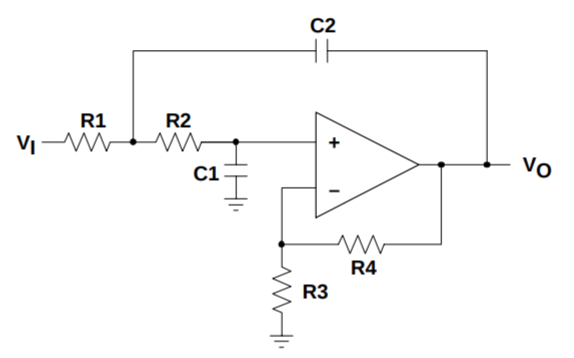
\includegraphics[scale=0.6]{figuras/fig-sallenKeyLPF}
			\caption{Sallen-Key Active Low Pass Filter \cite{texas1999sallenkey}}
			\label{fig:sallenKeyLPF}
		\end{figure}

		According to \cite{texas1999sallenkey}, this filter setup has a cutoff frequency defined by Equation \ref{eqn:sallenKeyTransferFunction}, quality factor (Q) defined by Equation \ref{eqn:sallenKeyQ}, gain(k) defined by Equation \ref{eqn:sallenKeyK} and cutoff frequency giver by Equation \ref{eqn:sallenKeyCutoffFrequency}.

		\begin{equation}\label{eqn:sallenKeyTransferFunction}
			H(s)=\frac{k}{s^{2} \cdot \left( R_{1} \cdot R_{2} \cdot C_{1} \cdot C_{2} \right) + s \cdot \left( R_{1} \cdot C_{1} + R_{2} \cdot C_{1} + R_{1} \cdot C_{2} \cdot \left( 1 - k \right) \right) + 1} 
		\end{equation}

		\begin{equation}\label{eqn:sallenKeyQ}
			Q=\frac{\sqrt{R_{1} \cdot R_{2} \cdot C_{1} \cdot C_{2}}}{R_{1} \cdot C_{1} + R_{2} \cdot C_{1} + R_{1} \cdot C_{2} \cdot \left( 1 - k \right)}
		\end{equation}

		\begin{equation}\label{eqn:sallenKeyK}
			k=1 + \frac{R_{4}}{R_{3}}
		\end{equation}

		\begin{equation}\label{eqn:sallenKeyCutoffFrequency}
			f_{c}=\frac{1}{2 \cdot \pi \sqrt{R_{1} \cdot R_{2} \cdot C_{1} \cdot C_{2}}} 
		\end{equation}


		As explained in Subsection \ref{ssec:filterCharacteristicsDefinition}, we need a gain of $k=2$ in the passing band. A useful design strategy is to set $R_{1}= m \cdot R$, $R_{2}=R$, $C_{1}=C$ and $C_{2}= n \cdot C$. Replacing this values in Equation \ref{eqn:sallenKeyQ} gives a new Equation \ref{eqn:sallenKeyQ2}.

		\begin{equation}\label{eqn:sallenKeyQ2}
			Q=\frac{\sqrt{m \cdot n}}{m + 1 - m \cdot n}
		\end{equation}

		The quality factor of a Sallen-Key filter is influenced by the gain (k) and defines the dB gain on the cutoff frequency, ideally this factor should be closer as possible to $\frac{\sqrt{2}}{2}$ \ref{dorfSvodoba2014}. Setting a arbitrary value of $m=2$, the ideal value of $Q=\frac{\sqrt{2}}{2}$ and using Equation \ref{eqn:sallenKeyQ2} it is possible to calculate a $n=0,6771$. It is possible to simplify Equation \ref{eqn:sallenKeyCutoffFrequency} using the same method used to simplify Equation \ref{eqn:sallenKeyQ} to \ref{eqn:sallenKeyQ2}. Using this method will produce Equation \ref{eqn:sallenKeyRC} that will be used to determine the $R \cdot C$ constant that will be later used to define the resistors and capacitor values of our filter. 

		\begin{equation}\label{eqn:sallenKeyRC}
			R \cdot C = \frac{1}{2 \cdot \pi f_{c} \cdot \sqrt{m \cdot n}}
		\end{equation}

		Using the previously calculated values for \textit{m}, \textit{n}, \textit{$f_{c}$} and Equation \ref{eqn:sallenKeyRC} wil give us a $R \cdot C = 3.50115 \cdot 10^{-5}$. Setting a arbitrary value of $R=10 \cdot 10^{3}$ will lead to $C=3.5 \cdot 10^{-9}$. Using the relations: $R_{1}= m \cdot R$, $R_{2}=R$, $C_{1}=C$ and $C_{2}= n \cdot C$ and the commercial resistors and capacitors values from \cite{burgess2015pwm}, will produce the following values: $R_{1}= 20k\Omega$, $R_{2}=10k\Omega$, $C_{1}=3600pF$ and $C_{2}= 2700pF$. If theese values are used in Equations \ref{eqn:sallenKeyQ} and \ref{eqn:sallenKeyCutoffFrequency}, we will have a  quality factor of 0.8164 and a cutoff frequency of 3609.71, both which are quite close from the ideal ones.
\par
		The last calculation remaining is the one to define $R_{3}$ and $R_{4}$ in order to guarantee a gain (k) equal to two. Looking at Equation \ref{eqn:sallenKeyK}, in order to reach a \textit{k} value equal to two, the only requirement is so $R_{3}$ equals to $R{4}$, so let's arbitrary set $R_{3}=R_{4}=10k\Omega$.

	\subsection{Final Circuit}

		Based on all the previously calculations and on \cite{texas1999sallenkey}, the final circuit will be the one in Figure \ref{fig:pwmToSpeedReferenceCircuit}. It was also added two Schottky Diodes for protection as \cite{walshAD} shows how to.

		\begin{figure}[htbp]
			\centering
				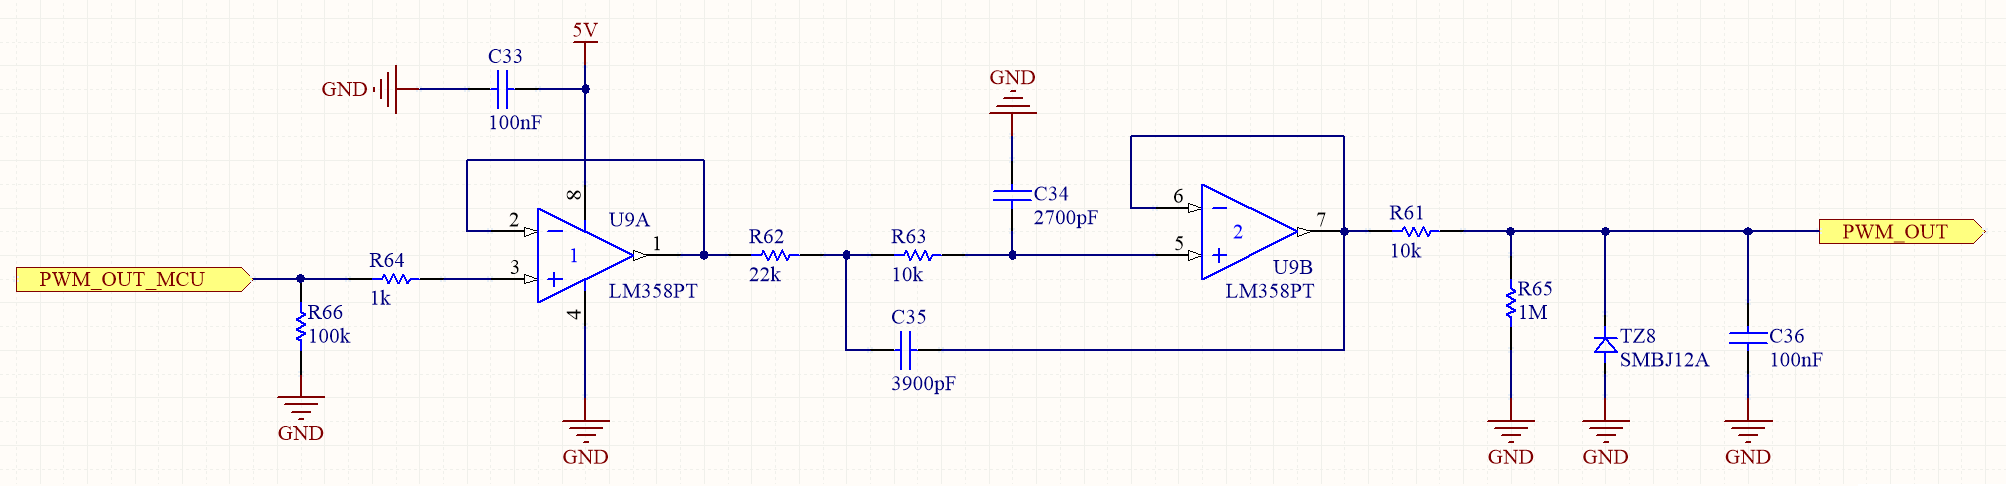
\includegraphics[scale=0.4]{figuras/fig-pwmToSpeedReferenceCircuit}
			\caption{PWM to Speed Reference Circuit}
			\label{fig:pwmToSpeedReferenceCircuit}
		\end{figure}



	\section{Hardware Interface Between Microcontroller and Computer}

	\subsection{USB and UART}
		Nowadays most computers do not have a serial port connector \cite{serialPortNeverSayDie}, the majority of communications with peripherals are done through USB ports. The choosen microcontroller for this project (as discussed on Section \ref{sec:mcu-hw}) does not have USB interface, only UART. 

		As it was explained in Sections \ref{sssec:usb} and \ref{sssec:uart}, USB communication protocol is half-duplex, UART protocol is full-duplex though. While USB is composed of a differential pair of data wires, UART has one wire for receiving and another one for transmitting information. 

		In order to make this project compatible with most of modern computers, there is the need to have a USB to UART converter circuit.

	\subsection{Conversion Circuit}

		The issue discussed in the previous section is not a new thing, so there are loads of integrated solutions to solve this issue \cite{usbSerialAdapter}. The choosen one was the Microchip's MCP2221A \cite{mcp2221a-datasheet}, this is a USB to UART/I$^2$C converter chip, it emulates a virtual serial port on the computer, making it possible to communicate with the microcontroller UART ports just using a pair of capacitors and a resistor as Figure \ref{fig:mcp2221a-basic-circuit} shows.

		\begin{figure}[htbp]
			\centering
				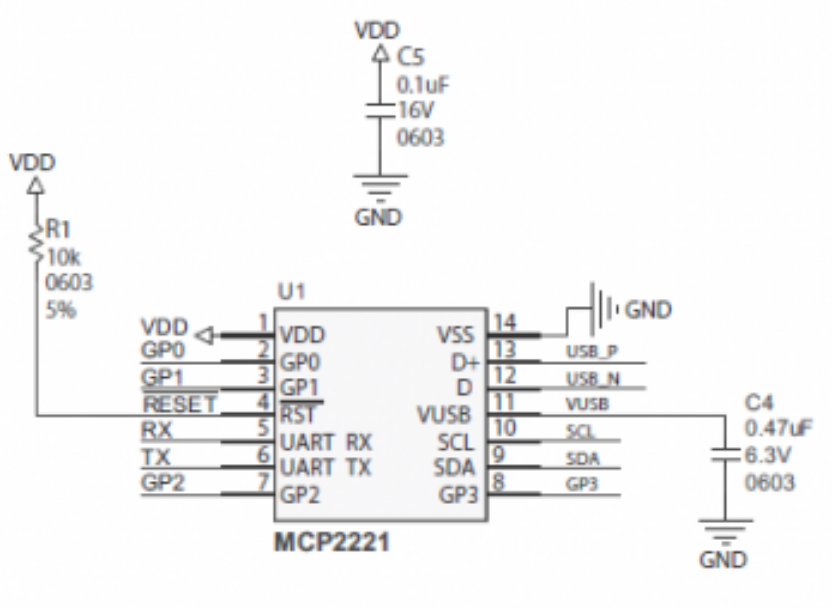
\includegraphics[scale=1]{figuras/fig-mcp2221a-basic-circuit}
			\caption{MCP2221A basic circuit \cite{mcp2221a-basic-circuit}}
			\label{fig:mcp2221a-basic-circuit}
		\end{figure}

		This chip already contains a internal 3V3 LDO in order to convert the 5V TTL level to the 3V3 standard level for USB data lines.


	\subsection{Circuit Protection}
		In order to ensure reliability on the circuit, ESD protection is needed, every connection between the circuit board and the outside world has the potential to pick unwanted noise and ESD, and USB is not exclued from that problem \cite{circuit-protection-usb}.

		High-frequency noise could be filtered using low pass filters in both data lines using discrete passive components. Moreover, the data lines could be protected from ESD using discrete TVS. The number of discrete componentes needed to filter and protect the lines makes a discrete-component-solution unpractical, expensive and spacious. Nowadays there are unexpensive integrated solutions in order to save space on the PCB, one of them is the ON Semiconductor STF202-22T1G. This IC is a USB Filter with ESD protection, as the datasheet \cite{stf202-22t1g-datasheet} says: \textit{"This device is designed for applications requireing Line Termination, EMI filtering and ESD protection"}, making it more than ideal for this project. The STF202-22T1G internal circuit can be seen on Figure \ref{fig:stf202-22t1g-sch}.

		\begin{figure}[htbp]
			\centering
				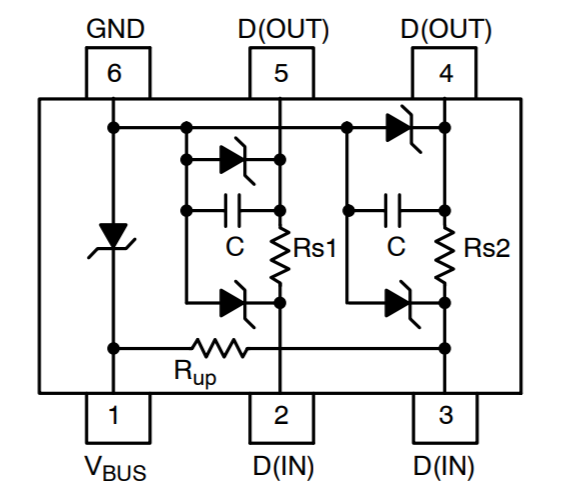
\includegraphics[scale=1]{figuras/fig-stf202-22t1g-sch}
			\caption{STF202-22T1G Internal Circuit \cite{stf202-22t1g-sch}}
			\label{fig:stf202-22t1g-sch}
		\end{figure}

	\subsection{Complete Circuit}

		For the final circuit the STF202-22T1G was connected before the MCP2221A in order to protect and filter the data lines. Moreover, two external resistors were added to the serial communication lines (based on the Arduino Rev3 Schematic \cite{arduino-rev3-schematic}). Figure \ref{fig:usb-uart-circuit} contains the final circuit.

		\begin{figure}[htbp]
			\centering
				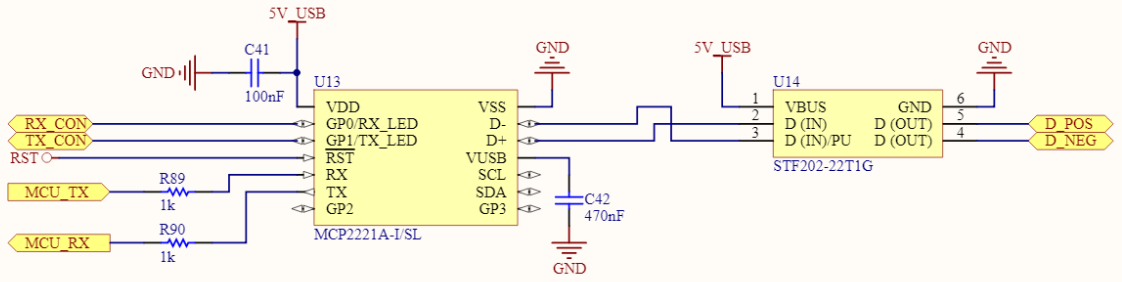
\includegraphics[scale=.8]{figuras/fig-usb-uart-circuit}
			\caption{USB/UART Converter Circuit \cite{usb-uart-circuit}}
			\label{fig:usb-uart-circuit}
		\end{figure}

		The \textit{TX CON} and \textit{RX CON} lines are used in other to indicate when the MCP2221A chip is repectively transmitting or receiving data. This lines drain current when data is transmitted or received and are used to blink LEDs in other parts of the circuit board. 

		Both capacitors are decoupling capacitors for the 5V and 3V3 lines. 
	\section{Digital Interfaces}\label{sec:digital-interfaces}

	All sensoring data was obtained using analog channels, some digital channels will be reserved on the board in order to provide another type of sensing and control.

	\subsection{Digital Outputs}\label{ssec:digital-outputs}

		\subsubsection{Low-side Driver}\label{sssec:digital-outputs-low-side-driver}

			Item \ref{itm:func-req-11} from Section \ref{sec:functionalRequirements} states that the system must have a digital output channel to control a relay). According to \cite{songle-relay-datasheet}, a standard 5V (MCU operating voltage, Section \ref{ssec:the-choosen-mcu}) relay will have a nominal current of 89.3mA, the microcontroller's datasheet \cite{atmega328p-datasheet} says that the maximum DC current per I/O pin is 40mA though. Hence it is not possible to activate a relay connected directly to a MCU's I/O pin.
			\par 
			In order to solve this a relay driver circuit needs to be used, in this case a low side mosfet driver similar to the one from Figure \cite{pmos-low-side-driver} will be used.

			\begin{figure}[htbp]
				\centering
				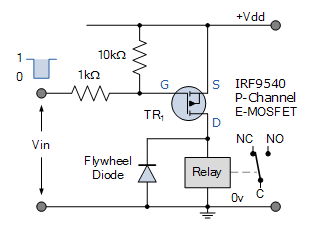
\includegraphics[scale=1]{figuras/fig-pmos-low-side-driver.png}
				\caption{PMOS low side driver \cite{pmos-low-side-driver}}
				\label{fig:pmos-low-side-driver}
			\end{figure}

			This is a low-side driver, when the PMOS is submitted to a high logic level (5V) in it's gate it will enter on the cutoff region and will not conduct current, hence not activating the relay. On the other hand, when a low logic level (0V) is applied to the device's gate it will enter the saturation region and will conduct current, hence activating the relay.

		\subsubsection{Digital Output Circuit}\label{sssec:digital-output-circuit}

			The digital output circuit will be very similar to the one from Figure \ref{fig:pmos-low-side-driver}. The power supply connected to the mosfet will be the 5V source (check Section \ref{sssec:5v-supply}), on the PMOS drain there will be a TVS diode (SMBJ12A from \textit{Littlefuse} \cite{smbj12a-datasheet}) (check Section \ref{sssec:tvsTransientProtection}), this TVS will protect the PMOS from reverse current and from overvoltages. Figure \ref{fig:digital-output-circuit} show the equivalent circuit for the digital output.

			\begin{figure}[htbp]
				\centering
				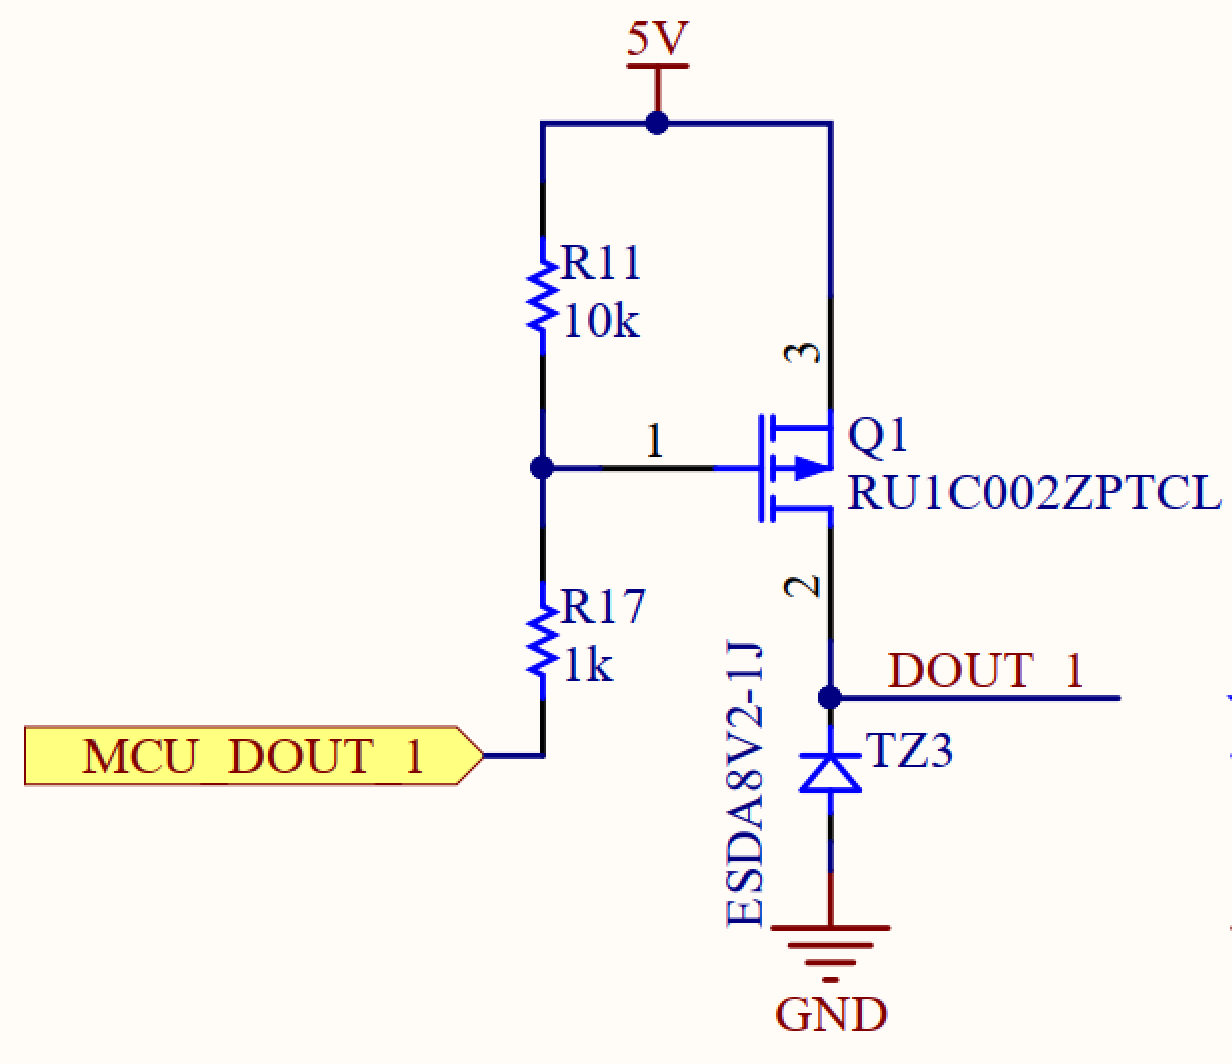
\includegraphics[scale=1]{figuras/fig-digital-output-circuit.png}
				\caption{Digital Output Circuit \cite{digital-output-circuit}}
				\label{fig:digital-output-circuit}
			\end{figure}

			The selected PMOS is the NDS332P from \textit{Fairchild} \cite{nds332p-datasheet}, it has a maximum operating continuos current of 1A, maximum gate threshold voltage of 1V, maximum drain-source voltage of 20V and maximum gate source voltage of $\pm$8V. It is adequate for this purpose. Resistor R7 is used to limit the magnitude of the current spike that can occur when a driver switches fast and has to charge or discharge a large gate capacitance. Resistor R5 is a pull-up for the gate, it will ensure that the PMOS will be in cutoff region if there is no input for the MCU. Resistor R8 is optional, for activating relays it is not needed, but other loads may require a pull-down, that is why it was placed on the PMOS drain. It was decided to keep any relay out of the board to save space. Moreover, keeping the relay out of the board gives room for using this digital output for other purposes.

	\subsection{Digital Inputs}\label{ssec:digital-inputs}

		This project does not have any requirement for digital inputs. However, in order to make the project more versatile for the future, it was decided to keep the space on the layout for soldering components to implement digital inputs. Figure \ref{fig:digital-input-circuit} show the circuit to interface the digital inputs.

			\begin{figure}[htbp]
				\centering
				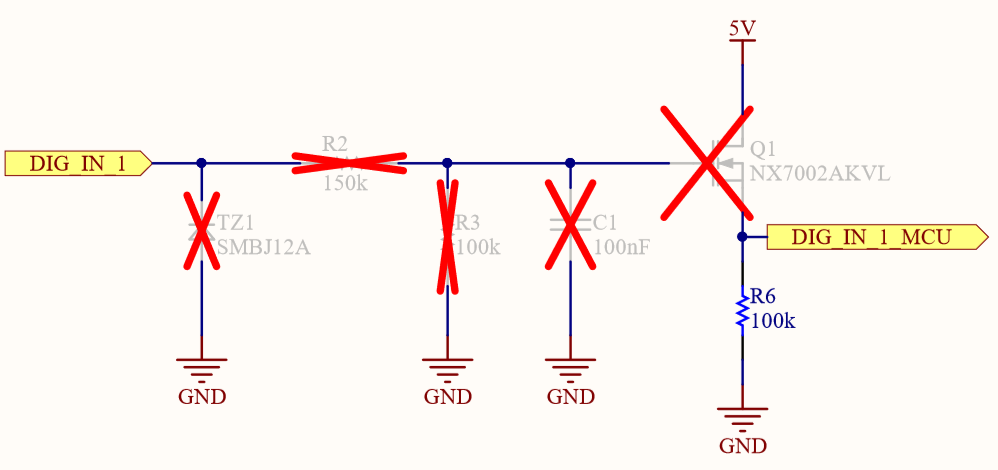
\includegraphics[scale=1]{figuras/fig-digital-input-circuit.png}
				\caption{Digital Input Circuit \cite{digital-input-circuit}}
				\label{fig:digital-input-circuit}
			\end{figure}

		The choosen NMOS was the NX7002AK from \textit{Nexperia} \cite{nx7002ak-datasheet}.This is a extremely versatile NMOS, it has a maximum drain source voltage of 60V, maximum gate-source voltage of $\pm$20V and maximum drain current of 300mA. This circuit is basically a buffer, it is used just to convert the state of the input signal to the MCU voltage limits. 

		This circuit is adjustable to different input voltages ($V_{IN}$), R4 and R3 creates a voltage divider and must be choosen according to Equation \ref{eqn:voltage-divider-digital-input}.

		\begin{equation}\label{eqn:voltage-divider-digital-input}
			2.1 < \frac{R4}{R4 + R3} \cdot V_{IN} < 5V
		\end{equation}

		For a 12V voltage input as an example, using $R_{2}=150k\Omega$ and $R_{3}=100k\Omega$ will produce a voltage at the gate equal to 4.8V, meeting the limits from Equation \ref{eqn:voltage-divider-digital-input}.

		This circuit also has a LPF formed by the combination of R3 and C10, it is used to filter any noise from the input. Equation \ref{eqn:1st-order-lpf-fc} is used to calculate the center frequency of this filter.

		\begin{equation}\label{eqn:1st-order-lpf-fc}
			f_{C} = \frac{1}{2 \cdot \pi \cdot R3 \cdot C10}
		\end{equation}

		The center frequency $f_{C}$ must be greater than the maximum input signal frequency to ensure operation.

		Finally, TZ1 is a TVS diode, it must be a TVS diode with a standoff voltage equal to the maximum input voltage. The layout was made to fit a SMBJ12CA from \textit{Littlefuse} \cite{smbj12a-datasheet}, this device has the DO-214AB footprint, any device with the same footprint can be soldered on it's pads.

	\section{LED driver circuits}\label{sec:led-driver-circuit}

	A keen aspect of a user operated system is the capability of the system to show useful and relevant feedback data to the user \cite{laurel1990art}. This system will have a high-layer software GUI in order to show processed data to the user as it was defined in Section \ref{sec:software-requirements} in Item \ref{itm:soft-req-6}. However, some direct hardware feedback is also useful, in this project the main hardware feature to show feedback are LEDs.
	\par
	The ideia is to have LEDs that will indicate in which stage of operation the system is. It was decided to make a separate LED circuit block in order to make changes on LED's types independent from the circuit they are giving feedback. The following sections will show and explain each functionality of the system that will have LED feedback. All LEDs will be directly connect to the power supplies and just their cathodes will be connect to the drivers circuit.
		
	\subsection{Serial Communication Leds}\label{ssec:serial-communication-leds}
		One important feature of the system is it's serial communication, this is the only way the MCU will communicate with the outside world, as was explained in Section \ref{sec:hardware-interface-between-mcu-and-computer}. In Section \ref{ssec:usb-uart-complete-circuit} it was said that nets \textit{TX$\_$CON} and \textit{RX$\_$CON} from Figure \ref{fig:usb-uart-circuit} are open drain input when the system is respectively transmitting and receiving serial data and high-impedance ports when they are not communicating.
		\par
		The system will have a LED to indicate transmission and another for reception of serial data, the solution to drive this LEDs will be the NTZD3152PT1H from \textit{ON Semiconductor} \cite{ntzd3152pt1h-datasheet}. This is a dual P-Channel mosfet in one IC with very low maximum\textit{Gate Threshold Voltage} ($V_{GS}=-1V$), as the USB/UART feedback pins drains current when communicating, by connecting theese pins to the Gate of theese PMOS it will be possible to control when the LEDs will be turned on. Figure \ref{fig:leds-uart} show this circuit configuration implemented.

		\begin{figure}[htbp]
			\centering
				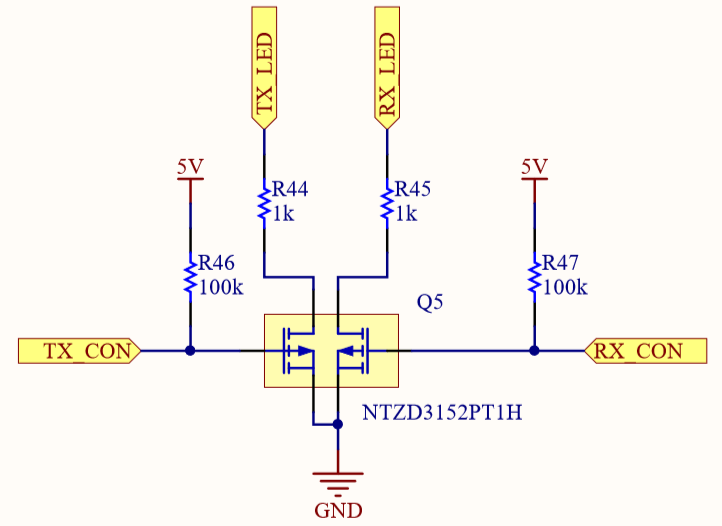
\includegraphics[scale=1.3]{figuras/fig-leds-uart.png}
			\caption{UART feedback LEDs driver \cite{leds-uart}}
			\label{fig:leds-uart}
		\end{figure}

		The resistors R44 and R45 are current limiting resistors, there value may vary with the choosen LEDs, so this 1k$\omega$ value is not necessary fixed. Resistors R46 and R47 have a relatively bigger resistance of 100k$\omega$ because they are pull-up resistos, they do not control current on that port, they were used just to guarantee that the voltage on the gate of the PMOS is higher than 1V (Gate-Source Threshold Voltae of the transistors according to the NTZD3152PT1H datasheet \cite{ntzd3152pt1h-datasheet}) when the UART/USB IC is turned off (in Section \ref{ssec:usb-uart-conversion-circuit} a possible scenario that the IC is not turned on is presented).

	\subsection{Sensor Disconnection and Acquisition Leds}\label{ssec:sensor-disconnection-acquisition-leds}	

		\subsubsection{Sensor Disconnection}\label{sssec:sensor-disconnection-leds}

			As it was defined in Item \ref{itm:func-req-14} from Section \ref{sec:functionalRequirements}, the system needs to be able to detect when a sensor is disconnected. Moreover, every sensor in this project has a net that goes to high-logic level (5V, according to Section {ssec:the-choosen-mcu}) and this signal can be used to activate LEDS to indicate wheter each sensor is connected or not.

		\subsubsection{Acquisition}\label{sssec:acquisition-led}

			The major funcition of this project is to make a acquisition system, so the major activity from the MCU is acquiring data. So, to give some feedback to the user a LED was reserved just for the MCU to indicate if the system is acquiring data or not. The control of this LED is controlled directly from the MCU, so if any extra functionality is desired to be implement, no hardware change will need to be carried out, just code.

		\subsubsection{Sensor Disconnection and Acquisition LED driver}\label{sssec:sensor-disconnection-and-acquisition-led-driver}

			As the sensor disconnection LEDs and the acquisition LED are all activated when high-logic level is present on their respective activation nets, the same solution can be applied. The choosen alternative to drive this LEDs is the TPL7407LAPWR from \textit{Texas Instruments} \cite{TPL7407LAPWR-datasheet}, it is a low-side driver than has a high-logic voltage level of 1.5V and a low-level voltage of 0.9V. The driver drains current when a high logic level is present at each channels activation port. This driver has seven channels and can drain up to 600mA per channel, making it more than ideal to drive LEDs. As this maximum drain current is quite high, if other devices such as relays and sirens can be connected instead of the LEDs without changing the hardware project, just changing the current limiting resistors. Figure \ref{fig:leds-sensor-disconnection-acquisition-circuit} shows the circuit to drive theese LEDs, resistors R30 to R36 are the current limiting resistors mentioned above and resistors R37 to R43 pull-down resistors used just to guarantee that the logic level will remain low (driver not draining current) if there is no definitive voltage input. The capacitor C10 is just a decoupling capacitor for the IC power supply recommended by the datasheet \cite{TPL7407LAPWR-datasheet}.

			\begin{figure}[htbp]
				\centering
					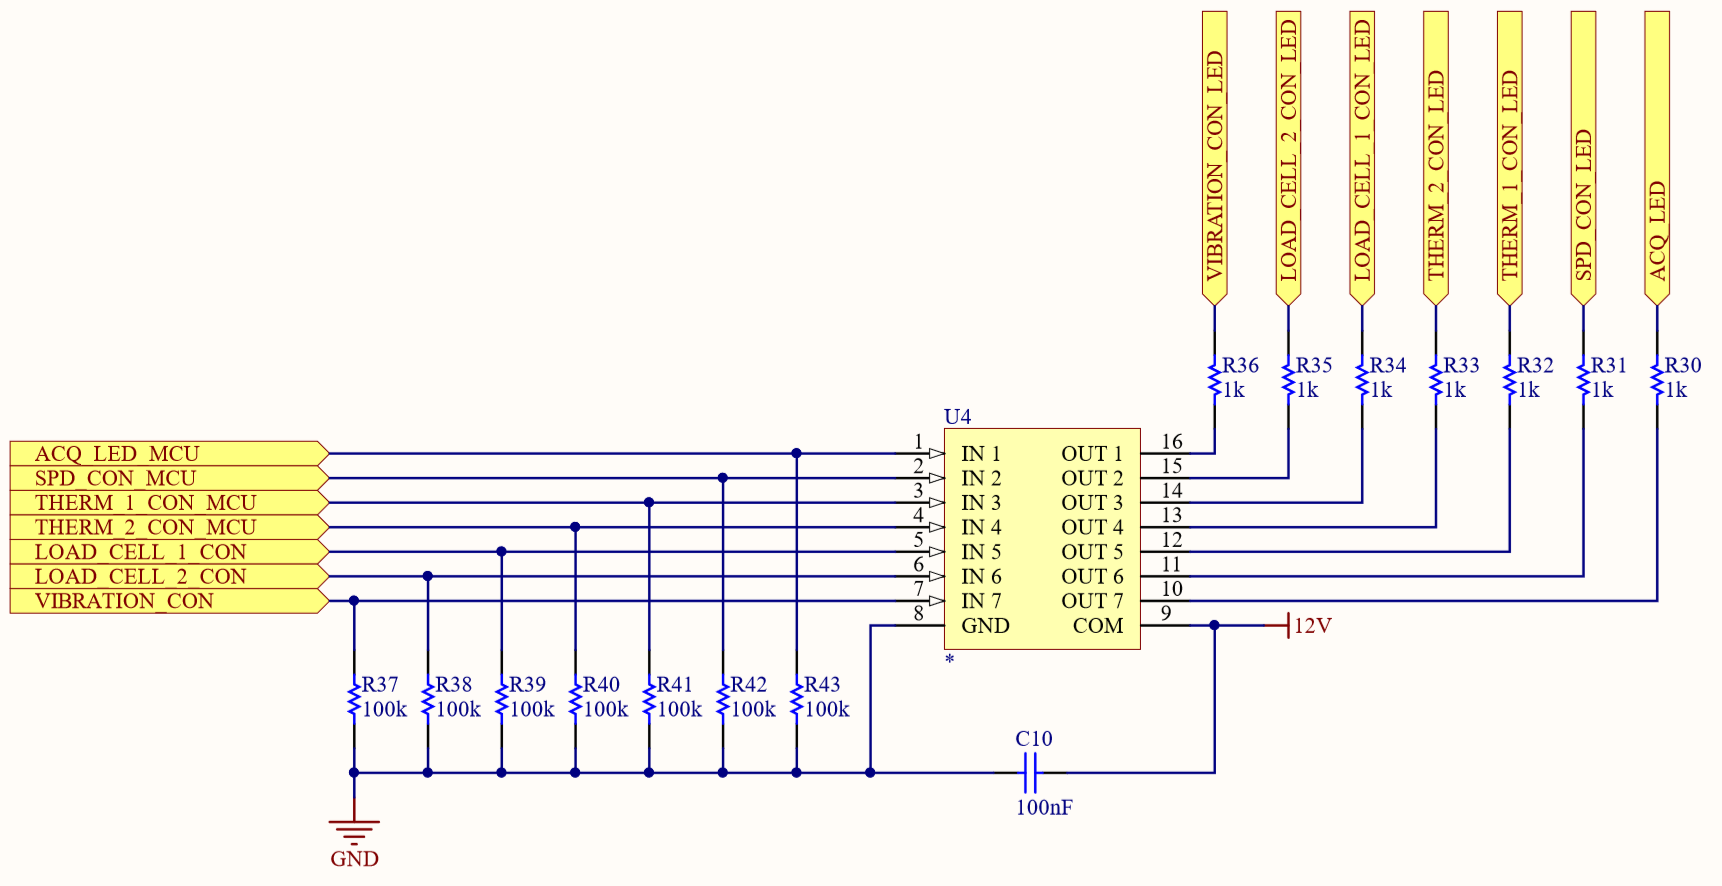
\includegraphics[scale=0.7]{figuras/fig-leds-sensor-disconnection-acquisition-circuit.png}
				\caption{Sensor Disconnection and Acquisition LED driver circuit \cite{leds-sensor-disconnection-acquisition-circuit}}
				\label{fig:leds-sensor-disconnection-acquisition-circuit}
			\end{figure}

	\subsection{Power Supplies Voltage LEDs}\label{ssec:power-supplis-voltage-leds}

		This is by far the simplest LED circuit, it is just current limiting resistors connected in series to the LEDs as Figure \ref{fig:power-supplies-leds} shows.

			\begin{figure}[htbp]
				\centering
					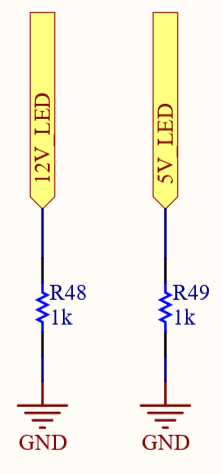
\includegraphics[scale=1.3]{figuras/fig-power-supplies-leds.png}
				\caption{Power Supplies Voltage LEDs Circuit \cite{power-supplies-leds}}
				\label{fig:power-supplies-leds}
			\end{figure}
	\section{Voltage Supplies}\label{sec:voltage-supplies}

	\subsection{Power Supplies}\label{ssec:power-supplies}
		In order to avoid any interference of the AC line, this project will work with a DC voltage input and any other necessary voltages will be acquainted from this higher input voltage supply.There are many different types of voltage regulators, nowadays the most common DC/DC being switching regulators. They are more efficient than linear regulators and consequently they waste less heat, the downside is the cost (due their consequently) and that they tend to have some ripple at the output \cite{schweber2017}. However, as this project does not aim radical cost management and as this ripple can be filtered, this type of voltage regulator was choosen for this project.

		\subsubsection{5V Supply}\label{sssec:5v-supply}
			Most of the choosen components for this project were choosen so they would be capable to work with single-supply of 5V. The choosen voltage regulator for the 5V supply was the TL2575-05 from \textit{Texas Instruments} \cite{tl2575-05-datasheet}, it has a output up to 1A, voltage drop ov 2V and typical efficiency of 88$\%$. Figure \ref{fig:tl2575-05-circuit} shows the circuit used for the 5V supply.

			\begin{figure}[htbp]
				\centering
					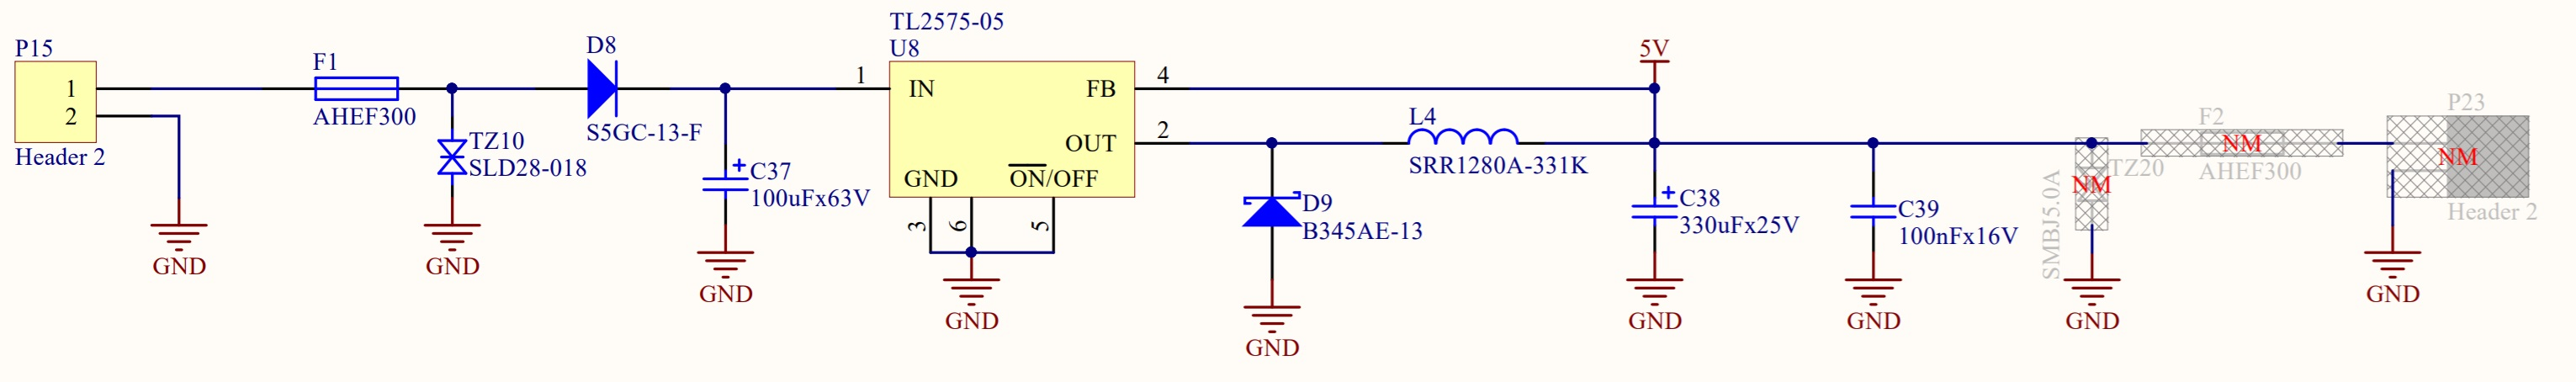
\includegraphics[scale=0.4]{figuras/fig-tl2575-05-circuit.png}
				\caption{5V Power Supply Circuit \cite{tl2575-05-circuit}}
				\label{fig:tl2575-05-circuit}
			\end{figure}

			The diode FM205-W from \textit{Rectron Semiconductor} \cite{fm205-2-datasheet} is used to protect the input of converter from inverse polarity. This diode has a maximum current of 2A, twice the maximum curret output of the regulator, so it will not interfere with the input current. Inductor L4 is fundamental for the device to work according to the datasheet. Capacitors C16 and C17 are a bypass capacitors recommended by the converter's datasheet. Diode D3 is a catch diode used to protect the converter from flyback currents from the inductor, the datasheet only specifies it should be a Schottky diode with maximum current at least the same as the maximum output current of the converter (1A). The choosen diode is FM5819-W from \textit{Rectron Semiconductor} \cite{fm5819-w-datasheet}.
			\par
			According to the datasheet this circuit has a input voltage from 7V to 40V.

		\subsubsection{12V Supply}\label{sssec:12v-supply}
			For the 12V supply the choosen regulator was LM2574-12 from \textit{Texas Instruments} \cite{lm2574-12-datasheet}, it has a output up to 500mA, voltage drop of 2V, and typical efficiency of $88\%$. Figure \ref{fig:lm2574-12-circuit} shows the circuit used for the 12V supply.

			\begin{figure}[htbp]
				\centering
					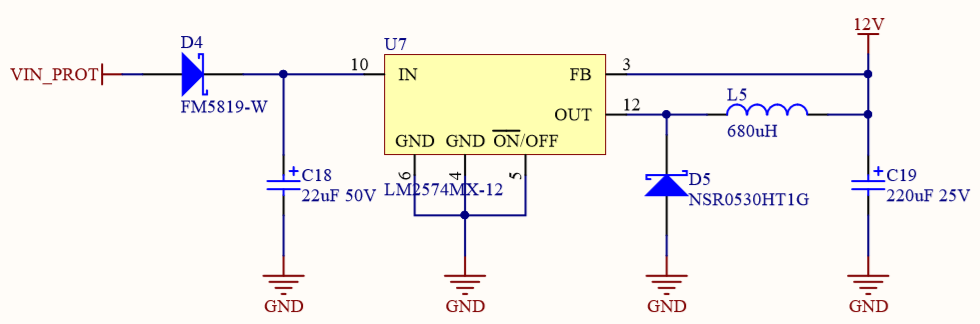
\includegraphics[scale=0.4]{figuras/fig-lm2574-12-circuit.png}
				\caption{5V Power Supply Circuit\cite{lm2574-12-circuit}}
				\label{fig:lm2574-12-circuit}
			\end{figure}	

			The diode FM5819-W from \textit{Rectron Semiconductor} \cite{fm5819-w-datasheet} is used to protect the input of converter from inverse polarity. This diode has a maximum current of 1A, twice the maximum curret output of the regulator, so it will not interfere with the input current. Inductor L5 is fundamental for the device to work according to the datasheet. Capacitors C18 and C19 are a bypass capacitors recommended by the converter's datasheet. Diode D5 is a catch diode used to protect the converter from flyback currents from the inductor, the datasheet only specifies it should be a Schottky diode with maximum current at least the same as the maximum output current of the converter (0.5A). The choosen diode is NSR0530HT1G from \textit{ON Semiconductor} \cite{NSR0530HT1G-datasheet}.
			\par
			According to the datasheet, this circuit has a input voltage from 14V to 40V.	

		\subsubsection{Voltage Input Protection}\label{sssec:voltage-input-protection}

			The voltage that goes to each of the switching voltage regulatores from Sections \ref{sssec:12v-supply} and \ref{sssec:5v-supply} is only protected against inverse polarity but not to overvoltage and overcurrent. Figure \ref{fig:input-protection-circuit} show the circuit used to protect the power supplies.

			\begin{figure}[htbp]
				\centering
					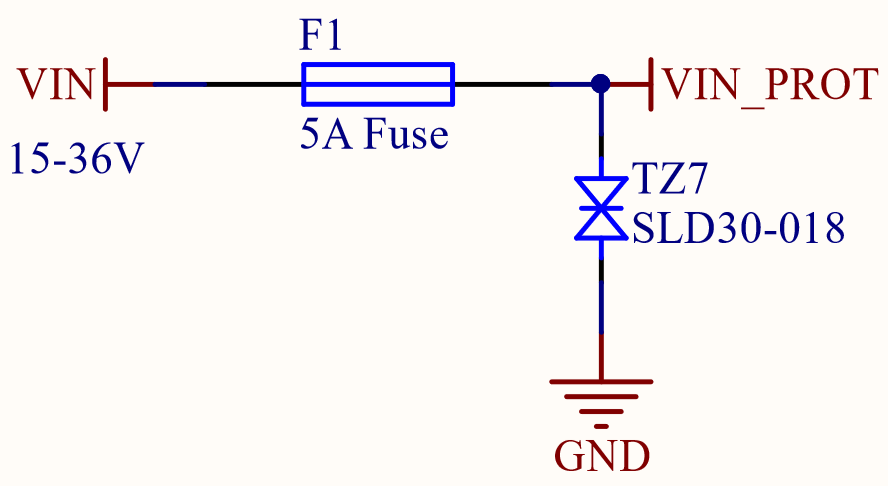
\includegraphics[scale=0.4]{figuras/fig-input-protection-circuit.png}
				\caption{Voltage Input Protection \cite{input-protection-circuit}}
				\label{fig:input-protection-circuit}
			\end{figure}

			TZ7 is a TVS diode used to protect the circuit against overvoltages. The choosen TVS is the SLD24-018, it has a standoff voltage of 24V and a maximum clamping voltage of 38.9 volts (check Section \ref{ssssec:tvsSelection}). Using this TVS limits the input voltage from 14-24V, in the other hand it ensures protection for the voltage regulators. F1 is a fuse with 5A rating, it will not protect the circuit from fast transients, this will be carried out by the TVS. It has the function to open the circuit when the TVS reaches its clamping voltage and protect the TVS.

	\subsection{Voltage References}\label{ssec:voltage-references}

		In this project any power supply that the precision and stability of the output voltage is more concerning than the maximum output current will be called a voltage reference.

		\subsubsection{10V Reference}\label{sssec:10v-reference}
			As it was explained in Section \ref{ssec:load-cell-signal-conditioning}, this voltage reference will be used to excite the load cells sensors of this project.
		\subsubsection{5V Reference}\label{sssec:5v-reference}
			This reference will be used by the MCU ADC, as said in Item \ref{itm:mcu-aref} from Section \ref{sssec:mcu-power-ports}, a ADC is only as good as it voltage reference. The choosen component for this reference was the LM4040DYM3-5.0-TR from \textit{Microchip} \cite{LM4040DYM3-5.0-TR-datasheet}. According to the datasheet, this voltage reference has a maximum tolerance of $\pm 58mV$ and has maximum operating output current of 15mA. Figure \ref{fig:LM4040DYM3-5.0-TR-circuit} shows to reference circuit.

			\begin{figure}[htbp]
				\centering
					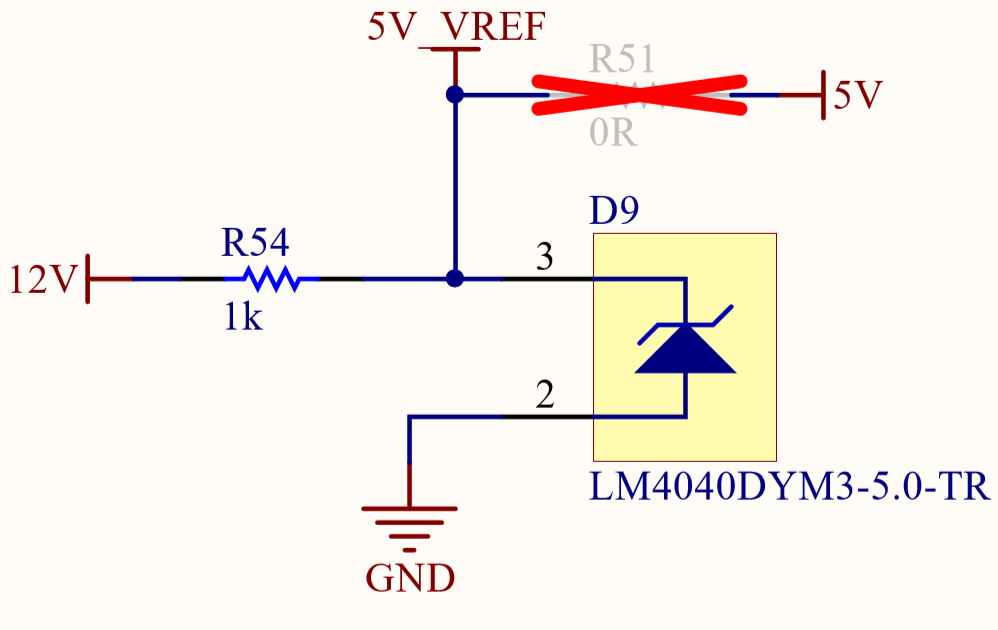
\includegraphics[scale=0.4]{figuras/fig-LM4040DYM3-5.0-TR-circuit.png}
				\caption{10V voltage reference circuit \cite{LM4040DYM3-5.0-TR-circuit}}
				\label{fig:LM4040DYM3-5.0-TR-circuit}
			\end{figure}

			The only external component needed

		\subsubsection{4V5 Reference}\label{sssec:4v5-reference}
		\subsubsection{1V Reference}\label{sssec:1v-reference}